\documentclass[t,xcolor={svgnames,table}]{beamer}

\mode<presentation>
\usetheme{Warsaw}
\useoutertheme{infolines} 
\usepackage{natbib}
\usepackage{fontspec}
\usepackage{lmodern}
\usepackage{amsmath}
\usepackage{amsfonts}
\usepackage{bbm}
\usepackage{bm}
\usepackage[font=small,labelfont=bf]{caption} % Required for specifying captions to tables and figures
\usepackage{nicefrac}
\usepackage{color}
\usepackage{perpage}
\usepackage{multirow}
\usepackage{multicol}
\usepackage{adjustbox}
\usepackage{tikz}
\usepackage{tikz-dependency}
\usepackage{tikz-qtree}
\usepackage{tikz,pgfplots,pgfplotstable}
\usepackage{pgf}
\usepackage{collcell}
\usepackage{booktabs}
\usepackage{color,soul}

\usetikzlibrary{arrows.meta,graphs,graphs.standard,graphdrawing,quotes,shapes}
\usegdlibrary{layered,trees}

\tikzset{
  invisible/.style={opacity=0},
  visible on/.style={alt={#1{}{invisible}}},
  alt/.code args={<#1>#2#3}{%
    \alt<#1>{\pgfkeysalso{#2}}{\pgfkeysalso{#3}} % \pgfkeysalso doesn't change the path
  },
}

\captionsetup{labelformat=empty}
\newcommand{\parser}[1]{TUPA\textsubscript{#1}}

\newfontfamily\hebfont[Script=Hebrew, Scale=MatchUppercase]{FreeSans}
\newcommand{\heb}[1]{\bgroup\textdir TRT\hebfont #1\egroup}

\newcommand{\ucca}[1]{\textcolor{gray}{\textbf{\textsf{#1}}}}
\newcommand{\sst}[1]{\textsc{#1}}
\newcommand{\lexcat}[1]{\textsl{#1}}

\definecolor{orange}{rgb}{1,0.5,0}
\definecolor{mdgreen}{rgb}{0.05,0.6,0.05}
\definecolor{Acolor}{HTML}{EC5D57} % poppy red
\definecolor{Pcolor}{HTML}{70BF41} % grass green
\definecolor{Scolor}{HTML}{51A7F9} % sky blue
\definecolor{Lcolor}{HTML}{B36AE2} % friendly purple
\definecolor{mdblue}{rgb}{0,0,0.7}
\definecolor{dkblue}{rgb}{0,0,0.5}
\definecolor{dkgray}{rgb}{0.3,0.3,0.3}
\definecolor{slate}{rgb}{0.25,0.25,0.4}
\definecolor{gray}{rgb}{0.5,0.5,0.5}
\definecolor{ltgray}{rgb}{0.7,0.7,0.7}
\definecolor{purple}{rgb}{0.7,0,1.0}
\definecolor{lavender}{rgb}{0.65,0.55,1.0}


\makeatletter
\pgfdeclareshape{vector}{
      \inheritsavedanchors[from={rectangle}]
      \inheritbackgroundpath[from={rectangle}]
      \inheritanchorborder[from={rectangle}]
      \foreach \x in {center,north east,north west,north,south,south east,south west,east,west}{
        \inheritanchor[from={rectangle}]{\x}
      }

    \backgroundpath{
      \pgftransformshift{\pgfpoint{-16pt}{-4pt}}
          \draw[rounded corners=2pt] (0,0) rectangle (32pt,8pt);
    }

    \beforebackgroundpath{
      \draw[step=8pt,help lines,-] (8pt,.1pt) grid (24pt,7.9pt);
    }
}
\pgfdeclareshape{vector}{
      \inheritsavedanchors[from={rectangle}]
      \inheritbackgroundpath[from={rectangle}]
      \inheritanchorborder[from={rectangle}]
      \foreach \x in {center,north east,north west,north,south,south east,south west,east,west}{
        \inheritanchor[from={rectangle}]{\x}
      }

    \backgroundpath{
      \pgftransformshift{\pgfpoint{-16pt}{-4pt}}
          \draw[rounded corners=2pt] (0,0) rectangle (32pt,8pt);
    }

    \beforebackgroundpath{
      \draw[step=8pt,help lines,-] (8pt,.1pt) grid (24pt,7.9pt);
    }
}
\makeatother


% for confusion matrix
\newcommand{\ApplyGradient}[1]{%
  \pgfmathsetmacro{\PercentColor}{(#1-0)/63.88}%
  \pgfmathsetmacro{\PercentInverse}{ifthenelse(\PercentColor > 70, 0, 100)}%
  %\textcolor{black!\PercentColor}{#1}
  \edef\x{\noexpand\cellcolor{red!\PercentColor}}\x\textcolor{black!\PercentInverse}{#1}%
}
\newcolumntype{R}{>{\collectcell\ApplyGradient}{c}<{\endcollectcell}}


\MakePerPage{footnote}

% Outline slides
\AtBeginSection[]
{\begin{frame} \frametitle{Outline} \tableofcontents[currentsection,currentsubsection] \end{frame}}


\begin{document}


\title[]{Universal Meaning Representation Parsing}
\author[Daniel Hershcovich]{Daniel Hershcovich \\ Joint work with Omri Abend and Ari Rappoport}
\date[November 29, 2019]{Seminar in Computational Linguistics \\ Uppsala University \\ November 29, 2019}

\begin{frame}
\titlepage
\end{frame}

\begin{frame}
\frametitle{What can we teach computers to do with language?}
\only<1>{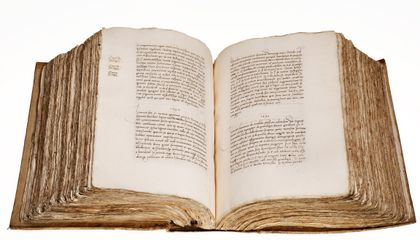
\includegraphics[width=\textwidth]{lostbook.jpg}}
\onslide<2>{Translate:}
\begin{center}
\onslide<2,6->{
  \fbox{\heb{דניאל עבר לקופנהגן אחרי שסיים את הלימודים}}
}

\only<2,4,5>{
  \fbox{After graduation, Daniel moved to Copenhagen}
}
\only<3,6->{
  \fbox{After graduation, \underline{Daniel} moved to \underline{Copenhagen}}
}
\end{center}

\vspace{-12mm}
  
\only<3>{
  Recognize \\ entities:

  \hspace{54mm} $\downarrow$ \hspace{27mm} $\downarrow$

  \hspace{49mm} Person \hspace{17mm} Location
}

\only<4>{
  \vspace{5mm}
  
  Infer:
}
  
\only<4>{
  \begin{center}
  $\downarrow$
  
  \fbox{Daniel graduated.}
  \end{center}
}

\only<5>{
  Simplify:
}
  
\only<5->{
  \vspace{6mm}
  
  \begin{center}  
  \fbox{Daniel graduated. Then Daniel moved to Copenhagen.}
  \end{center}
}

\only<6->{
  Neural models require the right \textit{inductive bias}.

  \begin{center}
    \begin{tikzpicture}[->]
    \tikzstyle{main}=[circle, minimum size=7mm, draw=black!80, node distance=12mm]
    \foreach \i in {1,3,7,9} {
        \node[main, fill=white!100] (h\i) at (\i,0) {};
        \node[main, fill=white!100] (o\i) at (\i.5,2) {};
    }
    \node (h5) at (5.5,0) {$\ldots$};
    \node (o5) at (5.5,2) {$\ldots$};
    \foreach \current/\next in {1/3,3/5,5/7,7/9} {
        \path (h\current) edge (h\next);
        \path (o\current) edge (o\next);
    }
    \foreach \i in {1,3,7,9} {
      \foreach \j in {1,3,7,9} {
        \path[gray!50] (h\i) edge (o\j);
      }
    }
    \path [alt=<7>{red,line width=1pt}{}] (h1) edge (o7);
    \end{tikzpicture}
  \end{center}
}

\end{frame}

\begin{frame}
\frametitle{Symbolic Structure Representation}
Relations between words or concepts.

\vfill

Example: {\color{DarkBlue}syntactic (UD)}/{\color{DarkRed}semantic (DM)}
bi-lexical dependencies.

\vfill

    \begin{adjustbox}{center}
    \begin{dependency}[line width=1.5pt]
        \begin{deptext}[column sep=1.5em,ampersand replacement=\^,font=\rmfamily]
          After \^ graduation \^ , \^ Daniel \^ moved \^ to \^ Copenhagen \\
        \end{deptext}
        \depedge[edge below,draw=DarkRed,edge unit distance=3ex]{1}{2}{ARG2}
        \depedge[edge below,draw=DarkRed,edge unit distance=3ex]{5}{4}{ARG1}
        \depedge[edge below,draw=DarkRed,edge unit distance=2ex, edge end x offset=-2pt]{1}{5}{ARG1}
        \deproot[edge below,draw=DarkRed,edge unit distance=3ex]{5}{top}
        \depedge[edge below,draw=DarkRed,edge unit distance=4ex, edge start x offset=-1pt, edge end x offset=3pt]{5}{7}{ARG2}
        \depedge[edge below,draw=DarkRed,edge unit distance=3ex, edge end x offset=5pt]{6}{5}{ARG1}
        \depedge[edge below,draw=DarkRed,edge unit distance=3ex]{6}{7}{ARG2}
        \depedge[draw=DarkBlue,edge unit distance=3ex]{2}{1}{case}
        \depedge[draw=DarkBlue,edge unit distance=3ex]{2}{3}{punct}
        \depedge[draw=DarkBlue,edge unit distance=3ex]{5}{4}{nsubj}
        \depedge[draw=DarkBlue,edge unit distance=3ex, edge end x offset=-2pt]{5}{2}{obl}
        \depedge[draw=DarkBlue,edge unit distance=3ex]{7}{6}{case}
        \deproot[draw=DarkBlue,edge unit distance=4ex]{5}{root}
        \depedge[draw=DarkBlue,edge unit distance=4ex]{5}{7}{obl}
    \end{dependency}    
    
    \end{adjustbox}
\end{frame}

\begin{frame}
    \frametitle{Meaning Representation}
Abstract away from detail that does not affect meaning:
\begin{center}    
    \fbox{\textrm{graduation}} $\approx$ \fbox{\textrm{graduated}}
    $\approx$ \fbox{\heb{סיים את הלימודים}} $\approx$ \fbox{\textrm{Abschluss}}
\end{center}

\pause\vfill

But capture useful distinctions, such as:
\vfill

\begin{minipage}{.38\textwidth}
\begin{itemize}
\item {\only<2>{\color{red}}Scenes and participants}
\item {\only<3>{\color{red}}Scene linkage}
\item {\only<4>{\color{red}}Multi-word chunking}
\end{itemize}
\end{minipage}
\begin{minipage}{.58\textwidth}\scalebox{.8}{
            \begin{tikzpicture}[level distance=21mm, sibling distance=1mm,
                every node/.append style={font=\rmfamily},
            	every circle node/.append style={fill=Indigo}]
                \begin{scope}[frontier/.style={distance from root=56mm},
                    edge from parent/.append style={nodes={font=\scriptsize}}]
                \Tree [.\node [circle] (root u) {};
                  \edge node[auto=right]{L}; \node[alt=<3>{text=red}{}] {Nach};
                  \edge node[auto=left]{H};
                  [.\node[circle](abschluss) {};
                    \edge node[auto=left]{P};
                    [.\node [circle] {};
                      \edge node[auto=right]{R}; \node {seinem};
                      \edge node[right]{C}; \node[alt=<2>{text=red}{}] (graduation) {Abschluss};
                    ]
                  ]
                  \edge node[auto=left]{H};
                  [.\node[circle]{};
                    \edge node[auto=left]{P};
                    [.\node[circle,xshift=8mm](zogum) {};
                      \edge node[auto=right]{}; \node[alt=<4>{text=red}{}] {zog};
                    ]
                    \edge node[right]{A}; \node[alt=<2>{text=red}{}] (Daniel) {Daniel};
                    \edge[draw=none]; \node[alt=<4>{text=red}{}] (um) {um};
                  ]
                ]
                \draw[dashed] (abschluss) to node[auto] {A} (Daniel);
                \draw (zogum.south) to node[left] {} (um);
                \end{scope}
            \end{tikzpicture}}
\end{minipage}\end{frame}


\section{UCCA}

\begin{frame}
\frametitle{Universal Conceptual Cognitive Annotation (UCCA)}
Supports rapid and intuitive annotation of linguistic semantic phenomena. \\
\only<1>{\citep{abend2013universal}}
\onslide<2->{
  Cross-linguistically applicable and stable \citep{sulem2015conceptual}.
}

\vfill

\begin{adjustbox}{center}
            \begin{tikzpicture}[level distance=7mm, sibling distance=6mm,
                every node/.append style={font=\rmfamily},
            	every circle node/.append style={fill=Indigo}]
                \begin{scope}[frontier/.style={distance from root=23mm},
                    edge from parent path={(\tikzparentnode.center)
                	.. controls +(0,-.25) and +(0,.25) .. (\tikzchildnode.north)},
                    edge from parent/.append style={nodes={font=\scriptsize}}]
                \Tree [.\node [circle] (root u) {};
                  \edge node [auto=right]{L}; \node (After u) {After};
                  \edge node[auto=left]{H};
                  [.\node [circle,xshift=8mm](graduation Daniel u) {};
                    \edge node[auto=right]{P}; \node (graduation u) {graduation};
                  ]
                  \edge node[auto=left]{H};
                  [.\node [circle](Daniel moved to Copenhagen u) {};
                    \edge node[auto=right]{A}; \node (Daniel u) {Daniel};
                    \edge node[auto=left]{P}; \node (moved u) {moved};
                    \edge node[auto=left]{A};
                    [.\node [circle](to Copenhagen u) {};
                      \edge node[auto=right]{R}; \node (to u) {to};
                      \edge node[auto=left]{C}; \node (Copenhagen u) {Copenhagen};
                    ]
                  ]
                ]
                \draw[dashed] (graduation Daniel u) to node[auto,style={font=\scriptsize}] {A} (Daniel u);
                \end{scope}
                \onslide<2->{
                  \begin{scope}[xshift=2cm,yshift=-58mm,grow'=up,level distance=9mm,
                      sibling distance=4mm, frontier/.style={distance from root=19mm},
                      edge from parent path={(\tikzparentnode.center) ..
                      controls +(0,.25) and +(0,-.25) .. (\tikzchildnode.south)},
                      edge from parent/.append style={nodes={font=\scriptsize}}]
                  \Tree [.\node [circle] (rootd) {};
                    \edge node[auto=left]{H};
                    [.\node [circle,xshift=-5mm] (Daniel siyem et halimudim d) {};
                      \edge node[auto=left]{P}; \node (halimudim d) {\heb{הלימודים}};
                      \edge node[auto=left]{F}; \node (et d) {\heb{את}};
                      \edge node[auto=right]{D}; \node (siyem d) {\heb{שסיים}};
                    ]
                    \edge node [auto=left,anchor=south east]{L}; \node (ahrei d) {\heb{אחרי}};
                    \edge node[auto=right]{H};
                    [.\node [circle] (hu avar lecopenhagen d) {};
                      \edge node[auto=left,anchor=south east]{A}; \node (lecopenhagen d) {\heb{לקופנהגן}};
                      \edge node[auto=left]{P}; \node (avar d) {\heb{עבר}};
                      \edge node[auto=right]{A}; \node (Daniel d) {\heb{דניאל}};
                    ]
                  ]
                  \draw[dashed] (Daniel siyem et halimudim d) to[out=-15,in=-150] node[above,style={font=\scriptsize}] {A} (Daniel d);
                  \end{scope}
                }\onslide<3>{
                  \begin{scope}[dashed,thick]
                    \draw[DarkRed] (After u) to[out=-45,in=135] (ahrei d);
                    \draw[DarkGreen] (graduation u) to[out=-90,in=100] (Daniel siyem et halimudim d);
                    \draw[DarkBlue] (Daniel u) -- (Daniel d);
                    \draw[orange] (moved u) to[out=-30,in=90] (avar d);
                    \draw[magenta] (to Copenhagen u) to[out=-90,in=70] (lecopenhagen d);
                  \end{scope}
                }
            \end{tikzpicture}
\end{adjustbox}
\end{frame}


\begin{frame}
\frametitle{UCCA Applications}
Semantics-based \textbf{evaluation} of
  \begin{itemize}
    \item Machine translation \citep{birch2016hume}.
    \item Text simplification \citep{sulem2018semantic}.
    \item {\only<2>{\color{red}}Grammatical error correction} \citep{choshen2018reference}.
  \end{itemize}

{\only<3>{\color{red}}Sentence splitting for text simplification} \citep{sulem2018simple}.

\pause

    \begin{minipage}{0.47\textwidth}
        \centering
        \scalebox{.9}{
                \begin{tikzpicture}[sibling distance=3mm, level distance=7mm,
                every node/.append style={font=\rmfamily},
            	every circle node/.append style={fill=black}]
                \begin{scope}[frontier/.style={distance from root=15mm},
            	edge from parent path={(\tikzparentnode.center) ..
                    controls +(0,-.25) and +(0,.25) .. (\tikzchildnode.north)}]
                \Tree [.\node [circle] (rootu) {};
                \edge node [auto=right]{}; \node (Heu) {He};
                \edge node[auto=right down]{}; \node (gve) {gve};
                \edge node[auto=right]{};
                [.\node [circle](an appleu) {};
                \edge node[auto=right]{}; \node (anu) {an};
                \edge node[auto=left]{}; \node (appleu) {apple};
                ]
                \edge node[auto=left]{};
                [.\node [circle](for daniel) {};
                \edge node[auto=right]{};\node (for) {for};
                \edge node[auto=left]{}; \node (daniel) {her};
                ]]
                \end{scope}
                \begin{scope}[yshift=-41mm,grow'=up,
                  frontier/.style={distance from root=12mm},
                  edge from parent path={(\tikzparentnode.center) ..
                  controls +(0,.25) and +(0,-.25) .. (\tikzchildnode.south)}]
                \Tree [.\node [circle] (rootd) {};
                \edge node [auto=left]{}; \node (Hed) {He};
                \edge node[auto=right]{}; \node (gave) {gave};
                \edge node[auto=right]{};\node (Daniel) {her};
                \edge node[auto=right]{};
                [.\node [circle] (an appled) {};
                \edge node[auto=left]{}; \node (and) {an};
                \edge node[auto=right]{}; \node (appled) {apple};
                ]
                ]
                \end{scope}
                \begin{scope}[dashed]
                \draw (Heu) -- (Hed);
                \draw (gve) -- (gave);
                \draw (Daniel) -- (daniel);
                \draw (anu) -- (and);
                \draw (appleu) -- (appled);
                \end{scope}
                \end{tikzpicture}
        }
    \end{minipage}
\pause
    \begin{minipage}{0.43\textwidth}
        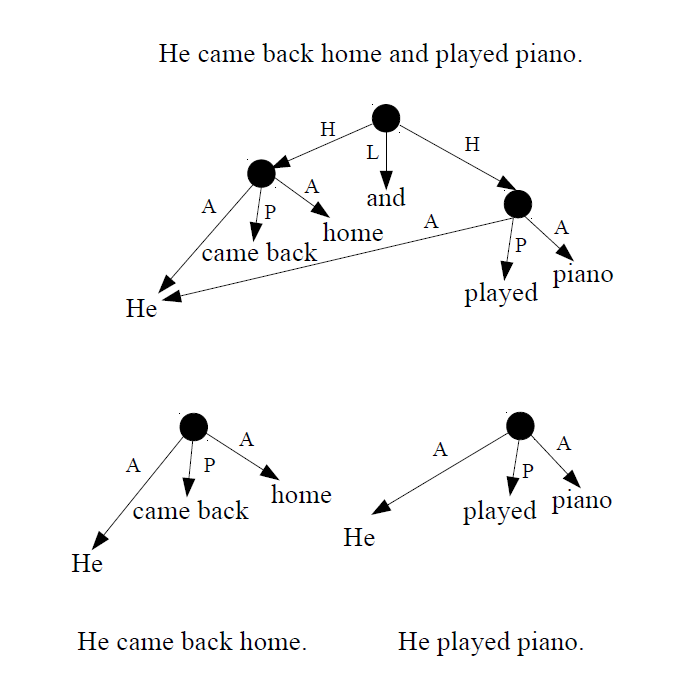
\includegraphics[width=1.2\textwidth,height=48mm]{ucca_simplification}  
    \end{minipage}
\end{frame}

\begin{frame}
\frametitle{Graph Structure}
UCCA structures are directed acyclic graphs (DAGs) with labeled edges. \\
Text tokens are terminals, complex units are {\color{blue} non-terminal nodes}. \\
\onslide<2->{
  Phrases may be {\color{red} discontinuous}.
}
\onslide<3->{
  \textit{Remote edges} enable {\color{orange} reentrancy}. \\
}

\hspace*{1cm}
\begin{tikzpicture}[level distance=18mm, sibling distance=28mm, ->, thick,
  level 2/.style={sibling distance=12mm},
  level 3/.style={sibling distance=18mm},
  edge from parent/.append style={nodes={font=\scriptsize}}]
  \tikzstyle{word} = [font=\rmfamily,color=black]
    \node (ROOT) [fill=blue, circle] {}
      child {node (They) [word] {They} edge from parent node[left] {A}}
      child {node [word] {thought} edge from parent node[left] {P}}
      child {node (abouttakingashortbreak) [fill=blue, circle] {}
      {
        child {node [word] {about} edge from parent node[left] {R}}
        child {node (takingabreak) [fill=blue, circle] {}
        {
          child {node [word] (taking) {taking} edge from parent node[above] {F}}
          child {node [word] (a) {a} edge from parent node[right] {F}}
          child {node [word] (short) {short} edge from parent[draw=none]}
          child {node [word] (break) {break} edge from parent node[right] {C}}
        } edge from parent node[right] {P} }
      } edge from parent node[right] {A} }
      ;
    \draw[bend left,dashed,->,visible on=<-2>] (abouttakingashortbreak) to node [auto] {\scriptsize A} (They);
    \draw[bend left,dashed,->,orange,very thick,visible on=<3->] (abouttakingashortbreak) to node [auto] {\scriptsize A} (They);
    \draw[bend left,->,visible on=<1>] (abouttakingashortbreak) to node [auto] {\scriptsize D} (short);
    \draw[red,very thick,->,visible on=<2>] (takingabreak.south) to node [auto] {} (taking.north);
    \draw[red,very thick,->,visible on=<2>] (takingabreak.south) to node [auto] {} (a.north);
    \draw[red,very thick,->,visible on=<2>] (takingabreak.south) to node [auto] {} (break.north);
    \draw[bend left,->] (abouttakingashortbreak) to node [auto] {\scriptsize D} (short);
    \node[visible on=<3->] at (6,-.4) {\Large ----- primary edge};
    \node[visible on=<3->] at (6,-1.4) {\Large - - - remote edge};
\end{tikzpicture}

\onslide<2->{
  \vspace{-26mm}
  \begin{adjustbox}{margin=1pt,frame,scale=.9}
    \begin{tabular}{c>{\small\it}l}
        P & Process \\
        A & Participant \\
        C & Center \\
        D & Adverbial \\
        R & Relator \\
        F & Function
    \end{tabular}
  \end{adjustbox}
}
\end{frame}


\begin{frame}
\frametitle{Structural Properties}
\noindent
\centering
\begin{minipage}{.5\linewidth}{\centering
(1) {\color{blue} non-terminal nodes}

\scalebox{.8}{
  \begin{tikzpicture}[level distance=12mm, sibling distance=16mm, ->, thick,
      every node/.append style={midway},
      edge from parent/.append style={nodes={font=\scriptsize}}]
    \node (ROOT) [fill=blue, circle] {}
      child {node [fill=blue, circle] {}
      {
        child {node {John} edge from parent node[left] {C}}
        child {node {and} edge from parent node[left] {N}}
        child {node {Mary} edge from parent node[right] {C}}
      } edge from parent node[left] {A} }
      child {node {went} edge from parent node[left] {P}}
      child {node {home} edge from parent node[right] {A}}
      ;
  \end{tikzpicture}
  }}
\end{minipage}
\hfill
\begin{minipage}{.48\linewidth}{\centering
(2) {\color{red} discontinuity}

\scalebox{.8}{
  \begin{tikzpicture}[level distance=12mm, sibling distance=2cm, ->, thick,
      every node/.append style={midway},
      edge from parent/.append style={nodes={font=\scriptsize}}]
    \node (ROOT) [fill=black, circle] {}
      child {node {John} edge from parent node[left] {A}}
      child {node [fill=black, circle] {}
      {
      	child {node {gave} edge from parent node[left] {C}}
      	child {node (everything) {everything} edge from parent[white]}
      	child {node {up} edge from parent node[right] {C}}
      } edge from parent node[right] {P} }
      ;
    \draw[bend right,->,red,very thick] (ROOT) to[out=-20, in=180] node [left] {\scriptsize A} (everything);
  \end{tikzpicture}
  }}
\end{minipage}

\vfill
(3) {\color{orange} reentrancy}

\scalebox{.8}{
\begin{tikzpicture}[level distance=14mm, sibling distance=17mm, ->, thick,
    edge from parent/.append style={nodes={font=\scriptsize}}]
    \node (ROOT) [fill=black, circle] {}
      child {node (After) {After} edge from parent node[left] {L\;}}
      child {node (graduation) [fill=black, circle] {}
      {
        child {node {graduation} edge from parent node[left] {P}}
      } edge from parent node[left] {H} }
      child {node {,} edge from parent node[right] {U}}
      child {node (moved) [fill=black, circle] {}
      {
        child {node (Daniel) {Daniel} edge from parent node[left] {A}}
        child {node {moved} edge from parent node[left] {P}}
        child {node [fill=black, circle] {}
        {
          child {node {to} edge from parent node[left] {R}}
          child {node {Copenhagen} edge from parent node[right] {C}}
        } edge from parent node[right] {A} }
      } edge from parent node[right] {H} }
      ;
    \draw[dashed,->,orange,very thick] (graduation) to node [auto] {\scriptsize A} (Daniel);
\end{tikzpicture}}
\end{frame}

\begin{frame}
\frametitle{UCCA Data}
\begin{itemize}
 \item English Wikipedia articles (158K tokens).
 \item Jules Verne's \textit{Twenty Thousand Leagues Under the Sea} \\ (12K English tokens, 12K French tokens, 144K German tokens).
 \item English Web Treebank reviews (55K tokens).
\end{itemize}

\vfill
\begin{center}
  \begin{minipage}{.26\textwidth}
\includegraphics[width=\textwidth]{wikipedia.png}\end{minipage}
  \begin{minipage}{.3\textwidth}
\includegraphics[width=\textwidth]{squid.jpg}\end{minipage}
  \begin{minipage}{.3\textwidth}
\includegraphics[width=\textwidth]{five-stars.png}\end{minipage}
\end{center}
\end{frame}

\begin{frame}
\frametitle{Data Statistics}
\centering
\def\arraystretch{1.5}
\begin{tabular}{l|r|rrr|r}
    & \multicolumn{1}{c|}{Wiki} & \multicolumn{3}{c|}{20K} & \multicolumn{1}{c}{EWT} \\
    & \multicolumn{1}{c|}{en} & \multicolumn{1}{c}{en} & \multicolumn{1}{c}{fr} & \multicolumn{1}{c|}{de} & \multicolumn{1}{c}{en} \\
    \hline
    \# sentences&5,141&492&492&6,514&3,813 \\
    \# tokens&158K&12K&12K&144K&55K \\
    \hline
    \# {\color{blue} non-terminal nodes}&62,002&4,699&5,110&51,934&18,156 \\
    \% {\color{red}discontinuous}&1.71&3.19&4.64&8.87&3.87 \\
    \% {\color{orange}reentrant}&1.84&0.89&0.65&0.31&0.83 \\
    \hline
    \# edges&208,937&16,803&17,520&187,533&60,739 \\
    \% primary&97.40&96.79&97.02&97.32&97.32 \\
    \% remote&2.60&3.21&2.98&2.68&2.68
\end{tabular}
\end{frame}


\begin{frame}
\frametitle{UCCA Parsing}
\centering
They thought about taking a short break

\[\Downarrow\]

\scalebox{.8}{
\begin{tikzpicture}[level distance=15mm, sibling distance=2cm, ->, thick,
    every node/.append style={font=\rmfamily},
    edge from parent/.append style={nodes={font=\scriptsize}},
    edge from parent path={(\tikzparentnode.center) -- (\tikzchildnode.north)}]
    \node(ROOT)[fill=black, circle] at (3,0) {}
      child {node (They) {They} edge from parent node [left] {A}}
      child {node (thought) {thought} edge from parent node [left] {P}}
      child {node (abouttakingashortbreak) [fill=blue, circle] {} 
      { 
        child {node (to) {about} edge from parent node [right] {R}}
        child {node (takingabreak) [fill=red, circle] {}
        {
          child {node (take) {taking} edge from parent node [above] {F}}      
          child {node (a) {a} edge from parent node [right] {F}} 
          child {node (short) {short} edge from parent [draw=none]}
          child {node (break) {break} edge from parent node [above] {C}}  
        } edge from parent [draw=none]}
      } edge from parent [draw=none]}
      ;
    \draw(abouttakingashortbreak) to node [left] {\scriptsize P} (takingabreak); 
    \draw(ROOT) to node [left] {A} (abouttakingashortbreak);
    \draw[bend left,dashed] (abouttakingashortbreak) to node [auto] {A} (They);
    \draw[bend left] (abouttakingashortbreak) to node [auto] {\scriptsize D} (short);
\end{tikzpicture}}
\end{frame}


\begin{frame}
\frametitle{TUPA: Transition-based UCCA Parser}

Parses text $w_1 \ldots w_n$ to graph $G$ incrementally by applying transitions to the parser state,
consisting of: stack, buffer and constructed graph \citep*{hershcovich2017a}.

\pause
\vfill
Initial state:
\scalebox{.9}{
\begin{tikzpicture}[xscale=1.4,every node/.append style={font=\rmfamily,
                    anchor=west,text height=.6ex,text depth=0}, circle]
    \draw[xstep=1,ystep=.5,color=gray] (-.01,0) grid (1,.5);
    \node[style={font=\sffamily}] at (-.1,.8) {stack};
    \node[fill=black] at (.3,.25) {};
    \draw[xstep=1,ystep=.5,color=gray] (2,0) grid (9,.5);
    \node[style={font=\sffamily}] at (8,.8) {buffer};
    \node at (2,.2) {\small They};
    \node at (3,.2) {\small thought};
    \node at (4,.2) {\small about};
    \node at (5,.2) {\small taking};
    \node at (6,.2) {\small a};
    \node at (7,.2) {\small short};
    \node at (8,.2) {\small break};
\end{tikzpicture}}

\vfill
\pause
\parser{} transitions:

\{\textsc{Shift, Reduce, {\color{blue}Node$_X$}, Left-Edge$_X$, Right-Edge$_X$,}\\
\hspace{5mm}\textsc{{\color{orange}Left-Remote$_X$}, {\color{orange}Right-Remote$_X$}, {\color{red}Swap}, Finish}\}

\vfill
These transitions enable {\color{blue}non-terminal nodes}, {\color{orange}reentrancy} and {\color{red}discontinuity}.
\end{frame}

\begin{frame}
\frametitle{Training}
An \textit{oracle} provides the transition sequence given the correct graph:

\vfill
\centering
\scalebox{.8}{
\begin{tikzpicture}[level distance=15mm, sibling distance=2cm, ->, thick,
    every node/.append style={font=\rmfamily},
    edge from parent/.append style={nodes={font=\scriptsize}},
    edge from parent path={(\tikzparentnode.center) -- (\tikzchildnode.north)}]
    \node(ROOT)[fill=black, circle] at (3,0) {}
      child {node (They) {They} edge from parent node [left] {A}}
      child {node (thought) {thought} edge from parent node [left] {P}}
      child {node (abouttakingashortbreak) [fill=blue, circle] {} 
      { 
        child {node (to) {about} edge from parent node [right] {R}}
        child {node (takingabreak) [fill=red, circle] {}
        {
          child {node (take) {taking} edge from parent node [above] {F}}      
          child {node (a) {a} edge from parent node [right] {F}} 
          child {node (short) {short} edge from parent [draw=none]}
          child {node (break) {break} edge from parent node [above] {C}}  
        } edge from parent [draw=none]}
      } edge from parent [draw=none]}
      ;
    \draw(abouttakingashortbreak) to node [left] {\scriptsize P} (takingabreak); 
    \draw(ROOT) to node [left] {A} (abouttakingashortbreak);
    \draw[bend left,dashed] (abouttakingashortbreak) to node [auto] {A} (They);
    \draw[bend left] (abouttakingashortbreak) to node [auto] {\scriptsize D} (short);
\end{tikzpicture}}
\[\Downarrow\]
\begin{flushleft}
\footnotesize
\textsc{Shift}, \textsc{Right-Edge$_A$}, \textsc{Shift}, \textsc{Swap}, \textsc{Right-Edge$_P$}, \textsc{Reduce}, \textsc{Shift}, \textsc{Shift}, \textsc{Node$_R$}, \textsc{Reduce}, \textsc{Left-Remote$_A$}, \textsc{Shift}, \textsc{Shift}, \textsc{Node$_C$}, \textsc{Reduce}, \textsc{Shift}, \textsc{Right-Edge$_P$}, \textsc{Shift}, \textsc{Right-Edge$_F$}, \textsc{Reduce}, \textsc{Shift}, \textsc{Swap}, \textsc{Right-Edge$_D$}, \textsc{Reduce}, \textsc{Swap}, \textsc{Right-Edge$_A$}, \textsc{Reduce}, \textsc{Reduce}, \textsc{Shift}, \textsc{Reduce}, \textsc{Shift}, \textsc{Right-Edge$_C$}, \textsc{Finish}
\end{flushleft}
\end{frame}


\begin{frame}
\frametitle{Example: TUPA Transition Sequence}
\begin{minipage}[t][8mm][t]{\textwidth}
    $\Rightarrow$\textsc{
        \only<1>{Shift}\only<2>{Right-Edge$_A$}\only<3>{Shift}\only<4>{Swap}\only<5>{Right-Edge$_P$}\only<6>{Reduce}\only<7>{Shift}\only<8>{Shift}\only<9>{Node$_R$}\only<10>{Reduce}\only<11>{Shift}\only<12>{Left-Remote$_A$}\only<13>{Shift}\only<14>{Node$_C$}\only<15>{Reduce}\only<16>{Shift}\only<17>{Right-Edge$_P$}\only<18>{Shift}\only<19>{Right-Edge$_F$}\only<20>{Reduce}\only<21>{Shift}\only<22>{Swap}\only<23>{Right-Edge$_D$}\only<24>{Reduce}\only<25>{Swap}\only<26>{Right-Edge$_A$}\only<27>{Reduce}\only<28>{Reduce}\only<29>{Shift}\only<30>{Reduce}\only<31>{Shift}\only<32>{Right-Edge$_C$}\only<33>{Finish}
    }
\end{minipage}

\vfill

\scalebox{.9}{
\begin{tikzpicture}[xscale=1.4,every node/.append style={font=\rmfamily, thick,
                    anchor=west,text height=.6ex,text depth=0}]
    \begin{scope}[style={font=\sffamily}]
      \node at (-.1,.8) {stack};
      \node at (8,  .8) {buffer};
    \end{scope}
    \begin{scope}[xstep=1,ystep=.5,color=red,line width=1pt]
      \only<31>    \draw (-.01,0) grid (1,.5);
      \only<1,7>   \draw (.99, 0) grid (2,.5);
      \only<2,5,26>\draw (-.01,0) grid (2,.5);
      \only<3,8,11>\draw (1.99,0) grid (3,.5);
      \only<13,16> \draw (2.99,0) grid (4,.5);
      \only<18,21> \draw (3.99,0) grid (5,.5);
      \only<17>    \draw (1.99,0) grid (4,.5);
      \only<19>    \draw (2.99,0) grid (5,.5);
      \only<4>     \draw (3,   0) grid (4,.5);
      \only<9>     \draw (4,   0) grid (5,.5);
      \only<14>    \draw (5,   0) grid (6,.5);
      \only<22>    \draw (7,   0) grid (8,.5);
      \only<25>    \draw (6,   0) grid (7,.5);
      \only<23>    \draw (1.99,0) grid (4,.5);
      \only<32>    \draw (-.01,0) grid (2,.5);
      \only<12>    \draw (.99, 0) grid (3,.5);
    \end{scope}
    \begin{scope}[xstep=1,ystep=.5,color=gray]
      \only<6,27,29,31->         \draw (-.01,0) grid (1, .5);
      \only<-2,4-5,7,10,25-26,33>\draw (-.01,0) grid (2, .5);
      \only<3,8-9,11-12,15,24>   \draw (-.01,0) grid (3, .5);
      \only<13-14,16-17,20,22-23>\draw (-.01,0) grid (4, .5);
      \only<18-19,21>            \draw (-.01,0) grid (5, .5);
      \only<-2,4-6>              \draw (3,   0) grid (9,.5);
      \only<3,5-7,9-10>          \draw (4,   0) grid (9,.5);
      \only<8,11-12,14-15>       \draw (5,   0) grid (9,.5);
      \only<13,16-17,25-28>      \draw (6,   0) grid (9,.5);
      \only<18-20,22-24,29-30>   \draw (7,   0) grid (9,.5);
      \only<21,31>               \draw (8,   0) grid (9,.5);
    \end{scope}
    \begin{scope}[xstep=.1,ystep=.5,color=gray]
      \only<28,30> \draw (-.01,0) grid (.1,.5);
      \only<32->   \draw (8.89,0) grid (9.01,.5);
    \end{scope}
    \only<-27>      \node[fill=black, circle] at (.3, .25) {};
    \only<25-26>    \node[fill=blue,  circle] at (1.3,.25) {};
    \only<11-24>    \node[fill=blue,  circle] at (2.3,.25) {};
    \only<31->      \node[fill=red,   circle] at (.3, .25) {};
    \only<16-21>    \node[fill=red,   circle] at (3.3,.25) {};
    \only<9-10>     \node[fill=blue,  circle] at (4.3,.25) {};
    \only<14-15>    \node[fill=red,   circle] at (5.3,.25) {};
    \only<22-30>    \node[fill=red,   circle] at (7.3,.25) {};
    \only<29>       \node at (0,.2) {\small They};
    \only<1-3,7-24> \node at (1,.2) {\small They};
    \only<4-5>      \node at (1,.2) {\small thought};
    \only<3>        \node at (2,.2) {\small thought};
    \only<8-9>      \node at (2,.2) {\small about};
    \only<13-14>    \node at (3,.2) {\small taking};
    \only<18-19>    \node at (4,.2) {\small a};
    \only<21>       \node at (4,.2) {\small short};
    \only<22-23>    \node at (3,.2) {\small short};
    \only<32->      \node at (1,.2) {\small break};
    \only<4-6>      \node at (3,.2) {\small They};
    \only<25-28>    \node at (6,.2) {\small They};
    \only<-2>       \node at (3,.2) {\small thought};
    \only<-7>       \node at (4,.2) {\small about};
    \only<-12>      \node at (5,.2) {\small taking};
    \only<-17>      \node at (6,.2) {\small a};
    \only<-20>      \node at (7,.2) {\small short};
    \only<-31>      \node at (8,.2) {\small break};
\end{tikzpicture}}
\vfill
\fbox{
\begin{tikzpicture}[level distance=14mm, sibling distance=26mm, ->,
    every node/.append style={font=\rmfamily},
    edge from parent/.append style={nodes={font=\scriptsize}},
    edge from parent path={(\tikzparentnode.center) -- (\tikzchildnode.north)}]
    \node[anchor=west,style={font=\sffamily}] at (0,0) {graph};
    \node(ROOT)[fill=black, circle, visible on=<1->] at (3,0) {}
      child [visible on=<2->,alt=<2>{draw=red}{}] {node (They) {They} edge from parent node [left] {A}}
      child [visible on=<5->,alt=<5>{draw=red}{}] {node (thought) {thought} edge from parent node [left] {P}}
      child [visible on=<9->] {node (abouttakingashortbreak) [fill=blue, circle] {}
      {
        child [visible on=<9->,alt=<9>{draw=red}{}] {node (to) {about} edge from parent node [right] {R}}
        child [visible on=<14->] {node (takingabreak) [fill=red, circle] {}
        {
          child [visible on=<14->] {node (take) {taking} edge from parent node [above] {F}}
          child [visible on=<19->,alt=<19>{draw=red}{}] {node (a) {a} edge from parent node [right] {F}}
          child [visible on=<23->,alt=<23>{draw=red}{}] {node (short) {short} edge from parent [draw=none]}
          child [visible on=<32->,alt=<32>{draw=red}{}] {node (break) {break} edge from parent node [above] {C}}
        } edge from parent [draw=none]}
      } edge from parent [draw=none]}
      ;
    \draw[visible on=<17->,alt=<17>{draw=red}{}] (abouttakingashortbreak) to node [left] {\scriptsize P} (takingabreak);
    \draw[visible on=<26->,alt=<26>{draw=red}{}] (ROOT) to node [left] {\scriptsize A} (abouttakingashortbreak);
    \draw[bend left,dashed, visible on=<12->,alt=<12>{draw=red}{}] (abouttakingashortbreak) to node [auto] {\scriptsize A} (They);
    \draw[bend left, visible on=<23->,alt=<23>{draw=red}{}] (abouttakingashortbreak) to node [auto] {\scriptsize D} (short);
\end{tikzpicture}}
\end{frame}

\begin{frame}
\frametitle{\parser{} Model}
Learns to greedily predict transition based on current state.

\only<1>{

\vspace{1cm}

Features include:

\{words, parts of speech, syntactic dependencies, existing edge labels\} \\
from the stack and buffer + parents, children, grandchildren.

\vspace{5mm}
\begin{tikzpicture}
    \draw[xstep=1cm,ystep=5mm,color=gray] (-.01,0) grid (4,.5);
    \draw[xstep=1cm,ystep=5mm,color=gray] (5,0) grid (10,.5);
    \node[anchor=west] at (-.1,1) {stack};
    \node[anchor=west] at (8.9,1) {buffer};
    \foreach \i in {0.5,8.5,9.5} {
        \node[fill=gray, circle] at (\i,.25) {};
    }
    \foreach \i in {1.5,2.5,3.5,5.5,6.5,7.5} {
        \node[fill=black, circle] at (\i,.25) {};
    }
\end{tikzpicture}
}

\pause

\centering
\fbox{\scalebox{.65}{
\begin{minipage}{.6\textwidth}
\begin{tikzpicture}[xscale=1.3,every node/.append style={font=\rmfamily}]
    \node[anchor=west,style={font=\sffamily}] at (-1,.25){stack};
    \draw[xstep=1,ystep=.5,color=gray] (-.01,0) grid (4,.5);
    \node[fill=black, circle] at (.5,.25) {};
    \node[fill=blue, circle] at (2.5,.25) {};
    \node[anchor=west] at (1,.25) {\small They};
    \node[anchor=west] at (3,.25) {\small taking};
\end{tikzpicture}

\vspace{1cm}
\begin{tikzpicture}[xscale=1.3,every node/.append style={font=\rmfamily}]
    \node[anchor=west,style={font=\sffamily}] at (-1,.25){buffer};
    \draw[xstep=1,ystep=.5,color=gray] (-.01,0) grid (4,.5);
    \node[fill=red, circle] at (.5,.25) {};
    \node[anchor=west] at (1,.25) {\small a};
    \node[anchor=west] at (2,.25) {\small short};
    \node[anchor=west] at (3,.25) {\small break};
\end{tikzpicture}
\end{minipage}
\begin{minipage}{.4\textwidth}
\scalebox{.65}{
\begin{tikzpicture}[xscale=1.5,level distance=1cm, sibling distance=12mm, ->,
    every node/.append style={font=\rmfamily,
                    anchor=west,text height=.6ex,text depth=0},
    edge from parent/.append style={nodes={font=\scriptsize}},
    edge from parent path={(\tikzparentnode.center) -- (\tikzchildnode.north)}]
    \node[anchor=west,style={font=\sffamily}] at (3,0) {graph};
    \draw[color=gray] (.2,.3) rectangle (3.9,-3.2);
    \node(ROOT)[fill=black, circle] at (1.2,0) {}
      child {node (They) {They} edge from parent node [left] {A}}
      child {node {thought} edge from parent node [left] {P}}
      child {node (abouttakingashortbreak) [fill=blue, circle] {}
      {
        child {node {about} edge from parent node [left] {R}}
        child {node (takingabreak) [fill=red, circle] {}
        {
          child {node {taking} edge from parent node [above] {F}}
          child [opacity=0] {node {a} edge from parent node [right] {F}}
          child [opacity=0] {node (short) {short} edge from parent [draw=none]}
          child [opacity=0] {node {break} edge from parent node [right] {C}}
        } edge from parent [draw=none]}
      } edge from parent [draw=none]}
      ;
\end{tikzpicture}
}
\end{minipage}
}}

\scalebox{.65}{
\begin{tikzpicture}[->,every node/.append style={anchor=north,text height=2ex,text depth=0}]
    \tiny
    \tikzstyle{main}=[circle, minimum size=7mm, draw=black!80, node distance=12mm]
    \foreach \i/\word in {1/{They},3/{thought},5/{about},7/{taking},9/{a},11/{short},13/{break}} {
        \node (x\i) at (\i,-1.3) {\Large\textrm\word};
        \node[main, fill=white!100] (h\i) at (\i,0) {LSTM};
        \path (x\i) edge (h\i);
        \node[main, fill=white!100] (i\i) at (\i.5,.8) {LSTM};
        \path (x\i) edge [bend right] (i\i);
        \node[main, fill=white!100] (l\i) at (\i.5,2.3) {LSTM};
        \path (h\i) edge [bend left] (l\i);
        \path (i\i) edge (l\i);
        \node[main, fill=white!100] (k\i) at (\i,3.1) {LSTM};
        \path (i\i) edge [bend left] (k\i);
        \path (h\i) edge [bend left] (k\i);
    }
    \foreach \current/\next in {1/3,3/5,5/7,7/9,9/11,11/13} {
        \path (h\current) edge (h\next);
        \path (i\next) edge (i\current);
        \path (l\current) edge (l\next);
        \path (k\next) edge (k\current);
    }
    \node[main, fill=white!100] (mlp) at (7,4.6) {MLP};
    \foreach \i in {1,5,7,9} {
        \path (l\i) edge (mlp);
        \path (k\i) edge (mlp);
    }
    \coordinate (state) at (10.5,6.5);
    \path (state) edge [bend left] (mlp);
    \node (transition) at (7,5.8) {\large\textsc{Node}$_C$};
    \path (mlp) edge (transition);
\end{tikzpicture}
}
\end{frame}

\begin{frame}
\frametitle{Comparing to Existing Methods}
Using conversion-based approximation as baseline, \\
with bi-lexical DAG parsers and transition-based tree parsers.

\vfill
\begin{center}
    \begin{dependency}
    \begin{deptext}[column sep=1.5em,ampersand replacement=\^,font=\rmfamily, thick]
	They \^ thought \^ about \^ taking \^ a \^ short \^ break \\
    \end{deptext}
    \depedge{2}{1}{A}
    \depedge[dashed,edge start x offset=6pt,edge end x offset=-6pt,edge unit distance=3.5ex]{7}{1}{A}
    \depedge{7}{3}{R}
    \depedge{7}{4}{F}
    \depedge{7}{5}{F}
    \depedge{7}{6}{D}
    \depedge{2}{7}{A}
    \end{dependency}
    \captionof{figure}{UCCA bi-lexical DAG approximation.}
\end{center}
\end{frame}


\begin{frame}
\frametitle{Bi-lexical Graph Approximation}
\begin{enumerate}
 \item Convert UCCA to bi-lexical DAGs.
 \item Train bi-lexical parsers.
 \item Parse test set.
 \item Convert to UCCA.
 \item Evaluate.
\end{enumerate}

\vspace{-15mm}

\begin{minipage}{.225\textwidth}
  \vspace{1cm}
  \begin{flushright}
    \begin{tikzpicture}[<->]
      \draw [ultra thick,red] (1,1) to[out=180,in=90] (0,0);
    \end{tikzpicture}
  \end{flushright}
\end{minipage}
\begin{minipage}{.7\textwidth}
    \begin{tikzpicture}[level distance=13mm, sibling distance=17mm, ->, thick,
        every circle node/.append style={fill=black},
        edge from parent/.append style={nodes={font=\scriptsize}},
        edge from parent path={(\tikzparentnode.center) -- (\tikzchildnode.north)}]
      \tikzstyle{word} = [font=\rmfamily,color=black]
      \node (ROOT) [circle] {}
        child {node (After) [word] {After} edge from parent node[left] {L}}
        child {node (graduation) [circle] {}
        {
          child {node [word] {graduation} edge from parent node[left] {P}}
        } edge from parent node[left] {H} }
        child {node [word] {,} edge from parent node[right] {U}}
        child {node (moved) [circle] {}
        {
          child {node (John) [word] {John} edge from parent node[left] {A}}
          child {node [word] {moved} edge from parent node[left] {P}}
          child {node [circle] {}
          {
            child {node [word] {to} edge from parent node[left] {R}}
            child {node [word] {Copenhagen} edge from parent node[right] {C}}
          } edge from parent node[right] {A} }
        } edge from parent node[right] {H} }
        ;
      \draw[dashed,->] (graduation) to node [auto] {\scriptsize A} (John);
    \end{tikzpicture}
\end{minipage}

\vspace{-14mm}
\begin{flushleft}
    \begin{dependency}
    \begin{deptext}[column sep=.7em,ampersand replacement=\^,font=\rmfamily, thick]
	After \^ graduation \^ , \^ John \^ moved \^ to \^ Copenhagen \\
    \end{deptext}
    \depedge{2}{1}{L}
    \depedge{2}{3}{U}
    \depedge[dashed]{2}{4}{A}
    \depedge{5}{4}{A}
    \depedge{2}{5}{H}
    \depedge{7}{6}{R}
    \depedge{5}{7}{A}
    \end{dependency}
\end{flushleft}
\end{frame}


\begin{frame}
\frametitle{Evaluation}
\begin{adjustbox}{frame,scale=.75,center}
    \begin{tikzpicture}[level distance=12mm, sibling distance=15mm, ->,
        every circle node/.append style={fill=black},
        edge from parent/.append style={nodes={font=\scriptsize}},
        edge from parent path={(\tikzparentnode.center) -- (\tikzchildnode.north)}]
      \tikzstyle{word} = [font=\rmfamily,color=black]
      \node at (0,.7) {True (human-annotated) graph};
      \node (ROOT) at (0,0) [circle] {}
        child {node (After) [word] {After} edge from parent node[left] {L}}
        child {node (graduation) [circle] {}
        {
          child {node [word] {graduation} edge from parent node[left] {P}}
        } edge from parent node[left] {H} }
        child {node [word] {,} edge from parent node[right] {U}}
        child {node (moved) [circle] {}
        {
          child {node (John) [word] {John} edge from parent node[left] {A}}
          child {node [word] {moved} edge from parent node[left] {P}}
          child {node [circle] {}
          {
            child {node [word] {to} edge from parent node[left] {R}}
            child {node [word] {Copenhagen} edge from parent node[right] {C}}
          } edge from parent node[right] {A} }
        } edge from parent node[right] {H} }
        ;
      \draw[dashed,->] (graduation) to node [auto] {\scriptsize A} (John);
      \node at (8,.7) {Automatically predicted graph for the same text};
      \node (ROOT_) at (7,0) [circle] {}
        child {node (After_) [word] {After} edge from parent node[left] {L}}
        child {node (graduation_) [circle] {}
        {
          child[alt=<2>{red}{}] {node [word] {graduation} edge from parent node[left] {S}}
        } edge from parent node[left] {H} }
        child {node [word] {,} edge from parent node[right] {U}}
        child {node (moved) [circle,xshift=3mm,yshift=-7mm] {}
        {
          child {node (John_) [word] {John} edge from parent node[left] {A}}
          child {node [word] {moved} edge from parent node[left] {P}}
          child[alt=<2>{red}{}] {node [word] {to} edge from parent node[left] {F}}
          child[alt=<2>{red}{}] {node (Copenhagen_) [word] {Copenhagen} edge from parent node[right] {A}}
        } edge from parent node[right] {H} }
        ;
      \draw[dashed,->] (graduation_) to node [auto] {\scriptsize A} (John_);
      \draw[bend left,dashed,->,alt=<2>{red}{}] (graduation_) to[in=90] node [auto] {\scriptsize A} (Copenhagen_);
    \end{tikzpicture}
\end{adjustbox}
\vfill

\begin{enumerate}
  \item Match primary edges between the graphs by terminal yield and label.
  \item Calculate \textbf{precision, recall and F1} scores.
  \item Repeat for remote edges.
\end{enumerate}

\pause
\vfill
\begin{adjustbox}{center}
    \begin{tabular}{c|c|c}
        \multicolumn{3}{l}{Primary} \\
        \textbf{P} & \textbf{R} & \textbf{F1} \\ \hline
        $\frac69=67\%$ & $\frac6{10}=60\%$ & 64\%
    \end{tabular}
    \hspace{1cm}
    \begin{tabular}{c|c|c}
        \multicolumn{3}{l}{Remote} \\
        \textbf{P} & \textbf{R} & \textbf{F1} \\ \hline
        $\frac12=50\%$ & $\frac11=100\%$ & 67\%
    \end{tabular}
\end{adjustbox}
\end{frame}


\section{Cross-lingual Parsing}

\begin{frame}
\frametitle{SemEval 2019: Cross-lingual UCCA Parsing}
Shared task: parsing text to UCCA graphs \citep*{hershcovich2019shared}.
\begin{itemize}
\item Data: UCCA for English, French, German.
\item Baseline: TUPA.
\item Participants: 8 teams from 6 countries.
\end{itemize}
\end{frame}

\begin{frame}
    \begin{figure}
        \centering
        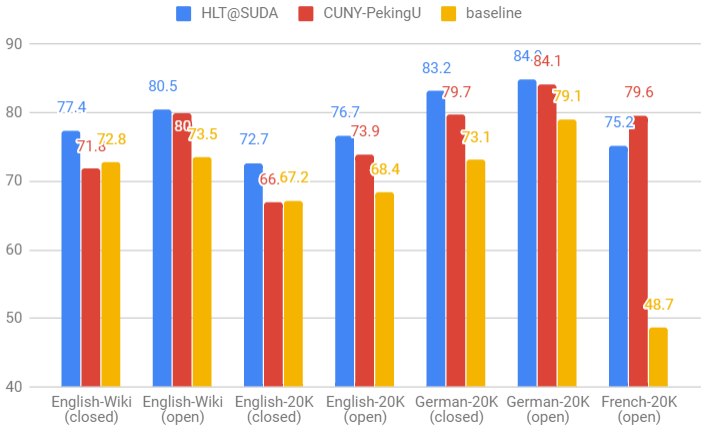
\includegraphics[width=\textwidth]{Capture}
    \end{figure}
\end{frame}



\begin{frame}
\frametitle{UCCA Graph Parsing as Constituent Tree Parsing}
Winning system: HLT@SUDA (Suzhou, China).

Neural constituency parser + multilingual BERT.
\begin{center}
%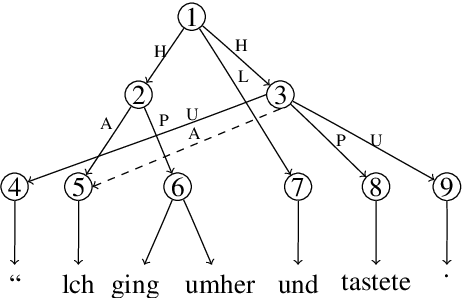
\includegraphics[width=.4\textwidth]{hltsuda1}$\to$
%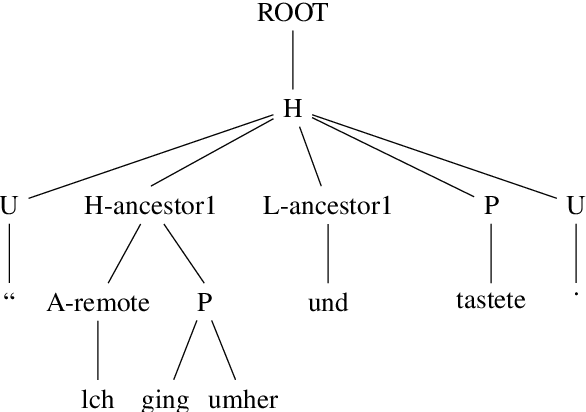
\includegraphics[width=.4\textwidth]{hltsuda2}
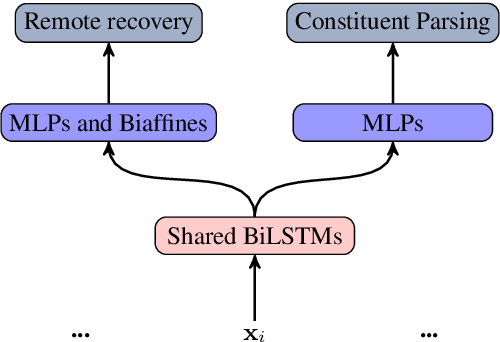
\includegraphics[width=.6\textwidth]{hltsuda3}
\end{center}
\end{frame}



\section{Cross-framework Parsing}


\begin{frame}
    \frametitle{Meaning Representations}

      \begin{flushright}
        \scalebox{.6}{
\begin{tikzpicture}[level distance=2cm, sibling distance=25mm, ->, draw=Indigo, thick]
    \node[font=\bf\sffamily\Huge,Indigo] at (-3,0) {UCCA};
    \node (ROOT) [fill=Indigo, circle] {}
      child {node (After) {After} edge from parent node[left] {L\;}}
      child {node (graduation) [fill=Indigo, circle] {}
      {
        child {node {graduation} edge from parent node[left] {P}}
      } edge from parent node[left] {H} }
      child {node {,} edge from parent node[right] {U}}
      child {node (moved) [fill=Indigo, circle] {}
      {
        child {node (Daniel) {Daniel} edge from parent node[left] {A}}
        child {node {moved} edge from parent node[left] {P}}
        child {node [fill=Indigo, circle] {}
        {
          child {node {to} edge from parent node[left] {R}}
          child {node {Copenhagen} edge from parent node[left] {C}}
        } edge from parent node[left] {A} }
      } edge from parent node[right] {H} }
      ;
    \draw[dashed,->] (graduation) to node [auto] {A} (Daniel);
\end{tikzpicture}
        }
      \end{flushright}
    
    \vspace{-23mm}
    
    \scalebox{.6}{
\begin{tikzpicture}[thick]
\node[font=\bf\sffamily\Huge,DarkGreen] at (0,6) {AMR};
\graph[layered layout, sibling distance=4cm, layer distance=2cm, nodes={ellipse,draw=DarkGreen}, edges={nodes={sloped}, DarkGreen}]{
a4 Copenhagen[as={Copenhagen}];
a2 Daniel[as={Daniel}];
a1[as={person}];
a0[as={move-01}];
a3[as={city}];
a2[as={name}];
a5[as={after}];
a4[as={name}];
a6[as={graduate-01}];

a1 ->  ["name"' above] a2;
a0 ->  ["ARG0"' above] a1;
a0 ->  ["ARG2"' above] a3;
a0 ->  ["time"' above] a5;
a3 ->  ["name"' above] a4;
a2 ->  ["op1"' above] a2 Daniel;
a5 ->  ["op1"' above] a6;
a4 ->  ["op1"' above] a4 Copenhagen;
};
\draw[->, above, DarkGreen] (a6) to node[sloped] {ARG0} (a1);
\end{tikzpicture}
      }
    \vspace{-15mm}
    
    \begin{flushright}
    \begin{minipage}{.01\textwidth}
      \begin{tikzpicture}
        \node[font=\bf\sffamily\Large,DarkRed] {DM};
      \end{tikzpicture}
    \end{minipage}
    \begin{minipage}{.6\textwidth}
        \rmfamily
        \scalebox{.7}{
\begin{dependency}[theme=simple,edge style={-{Latex[length=2mm]}, color=DarkRed},
            text only label, label style={above, color=DarkRed, font=\bf\ttfamily}, font=\small, thick]
    \begin{deptext}[column sep=1em,ampersand replacement=\^]
	After \^ graduation \^ , \^ Daniel \^ moved \^ to \^ Copenhagen \\
    \end{deptext}
    \deproot{5}{top}
    \depedge{1}{2}{ARG2}
    \depedge{1}{5}{ARG1}
    \depedge{5}{4}{ARG1}
    \depedge{6}{5}{ARG1}
    \depedge{6}{7}{ARG2}
\end{dependency}
    }
    \end{minipage}
    \end{flushright}
\end{frame}


\begin{frame}
\frametitle{Syntactic Representations}
    {\color{DarkBlue}\bf\sffamily\Large UD} (Universal Dependencies)
    
    \begin{center}
    \rmfamily
    \begin{dependency}[text only label, edge style={-{Latex[length=2mm]}, color=DarkBlue}, thick,
                       label style={above, color=DarkBlue, font=\bf\ttfamily}, font=\small]
    \begin{deptext}[column sep=.8em,ampersand replacement=\^]
    After \^ graduation \^ , \^ Daniel \^ moved \^ to \^ Copenhagen \\
    \end{deptext}
        \depedge{2}{1}{case}
        \depedge{2}{3}{punct}
        \depedge{5}{4}{nsubj}
        \depedge[edge end x offset=-2pt]{5}{2}{obl}
        \depedge{7}{6}{case}
        \deproot[edge unit distance=2.5ex]{5}{root}
        \depedge{5}{7}{obl}
    \end{dependency}
    \end{center}
\end{frame}


\begin{frame}
    \frametitle{Data}
    \fbox{UCCA training data is scarce}
    \begin{center}
    \begin{minipage}{.15\textwidth}
      (English)
    \end{minipage}
    \begin{minipage}{.7\textwidth}
    \pgfplotstableread[row sep=\\,col sep=&]{
    	corpus & total \\
        \color{DarkBlue} UD & 35791 \\
        \color{DarkRed} DM & 33964 \\
        \color{DarkGreen} AMR & 36521 \\
        \color{Indigo} UCCA & 5141 \\
        }\english
        \begin{tikzpicture}
        \begin{axis}[
        xbar stacked,
        width=10cm,
        height=39mm,
        xmin=0,
        xmax=60000,
        xtick=\empty,
        ytick=data,
        yticklabels from table={\english}{corpus},
        axis x line=none,
        ]
        \addplot [fill=Navy, point meta=explicit symbolic,
        nodes near coords align={anchor=west}] table [x=total,y expr=\coordindex,meta=total] {\english};
        \end{axis}
        \end{tikzpicture}
    \end{minipage}
    \end{center}
    
    \pause
    \vfill
    
    \begin{flushright}
        \fbox{and domains are limited.}
    \end{flushright}
    \begin{center}
    \begin{tabular}{llll}
        \color{Indigo} UCCA  & \color{DarkGreen} AMR  & \color{DarkRed} DM  & \color{NavyBlue} UD  \\
    	Wikipedia & blogs & news & blogs \\ books & news && news \\ reviews & emails && emails \\ & reviews && reviews \\ &&& Q\&A
    \end{tabular}
    \end{center}
\end{frame}

\def\convertedudgraduation{
  \begin{tikzpicture}[level distance=15mm, ->, draw=DarkBlue, thick,
      every node/.append style={sloped,anchor=south,auto=false,font=\scriptsize},
      level 1/.style={sibling distance=16mm},
      level 2/.style={sibling distance=13mm},
      edge from parent path={(\tikzparentnode.center) -- (\tikzchildnode.north)}]
    \tikzstyle{word} = [font=\rmfamily,color=black]
    \node (ROOT) [fill=DarkBlue,circle] {}
      child {node (after) [fill=DarkBlue,circle] {}
      {
        child {node [word] {After{\color{white}g}\quad\quad} edge from parent node {case}}
        child {node [word] {\quad graduation\quad\quad} edge from parent node {head}}
      } edge from parent node {obl}}
      child {node {}
      {
        child {node [word] (comma) {\quad,{\color{white}g}} edge from parent [draw=none]}
      } edge from parent [draw=none]}
      child {node {}
      {
        child {node [word] (Daniel) {Daniel{\color{white}g}} edge from parent [draw=none]}
      } edge from parent [draw=none]}
      child {node {}
      {
        child {node [word] (moved) {moved{\color{white}g}} edge from parent [draw=none]}
      } edge from parent [draw=none]}
      child {node (to) [fill=DarkBlue,circle] {}
      {
          child {node [word] {to{\color{white}g}} edge from parent node {case}}
          child {node [word] {Copenhagen{\color{white}g}} edge from parent node {head}}
      } edge from parent node {obl}}
      ;
      \draw (ROOT) to node {punct} (comma);
      \draw (ROOT) to node {nsubj} (Daniel);
      \draw (ROOT) to node {head} (moved);
  \end{tikzpicture}
}


\begin{frame}
\frametitle{Conversion}

\begin{minipage}{.04\textwidth}
\vspace{4mm}
\color{DarkGreen} AMR\\
\vspace{13mm}
\color{DarkRed} DM\\
\vspace{14mm}
\color{DarkBlue} UD
\end{minipage}
\begin{minipage}{.45\textwidth}
  \centering
  \scalebox{.6}{
  \begin{tikzpicture}[->,draw=DarkGreen,
      every node/.append style={sloped,anchor=south,auto=false,font=\tiny},
      level 1/.style={level distance=14mm,sibling distance=26mm},
      level 2/.style={level distance=13mm},
      level 3/.style={level distance=12mm}]
    \node (ROOT) [draw=DarkGreen,ellipse] {move-01}
      child {node [draw=DarkGreen,ellipse] {city}
      {
        child {node [draw=DarkGreen,ellipse] {name}
        {
            child {node [draw=DarkGreen,ellipse] {"Copenhagen"} edge from parent node {op1} }
        } edge from parent node {name} }
      } edge from parent node {ARG2} }
      child {node [draw=DarkGreen,ellipse] {after}
      {
            child {node (graduation) [draw=DarkGreen,ellipse] {graduate-01} edge from parent node {op1} }
      } edge from parent node {time} }
      child {node (Daniel) [draw=DarkGreen,ellipse] {person}
      {
        child {node [draw=DarkGreen,ellipse] {name}
        {
            child {node [draw=DarkGreen,ellipse] {"Daniel"} edge from parent node {op1} }
        } edge from parent node {name} }
      } edge from parent node {ARG0} }
      ;
      \draw (graduation) to node {ARG0} (Daniel);
  \end{tikzpicture}
  }
  
  \vspace{5mm}
  \scalebox{.6}{
    \begin{dependency}[theme=simple,text only label, font=\small, edge style={color=DarkRed},
                       label style={above, color=DarkRed, font=\bf\ttfamily}]
    \begin{deptext}[column sep=.8em,ampersand replacement=\^]
    After \^ graduation \^ , \^ Daniel \^ moved \^ to \^ Copenhagen \\
    \end{deptext}
        \depedge{1}{2}{ARG2}
        \depedge{5}{4}{ARG1}
        \depedge[edge end x offset=-2pt]{1}{5}{ARG1}
        \deproot[edge unit distance=3.5ex]{5}{top}
        \depedge[edge start x offset=-1pt, edge end x offset=3pt]{5}{7}{ARG2}
        \depedge[edge end x offset=5pt]{6}{5}{ARG1}
        \depedge{6}{7}{ARG2}
    \end{dependency}
    }
    
  \vspace{5mm}
  \scalebox{.6}{
    \begin{dependency}[text only label, edge style={color=DarkBlue},
                       label style={above, color=DarkBlue, font=\bf\ttfamily}, font=\small]
    \begin{deptext}[column sep=.8em,ampersand replacement=\^]
    After \^ graduation \^ , \^ Daniel \^ moved \^ to \^ Copenhagen \\
    \end{deptext}
        \depedge{2}{1}{case}
        \depedge{2}{3}{punct}
        \depedge{5}{4}{nsubj}
        \depedge[edge end x offset=-2pt]{5}{2}{obl}
        \depedge{7}{6}{case}
        \deproot[edge unit distance=2.5ex]{5}{root}
        \depedge{5}{7}{obl}
    \end{dependency}
    }

\end{minipage}
\begin{minipage}{.02\textwidth}
\vspace{7mm}
\Rightarrow
\vspace{16mm}
\Rightarrow
\vspace{20mm}
\Rightarrow
\end{minipage}
\begin{minipage}{.45\textwidth}

  \centering
  \scalebox{.6}{
  \begin{tikzpicture}[level distance=16mm, ->, draw=DarkGreen, thick,
      every node/.append style={sloped,anchor=south,auto=false,font=\scriptsize},
      level 1/.style={sibling distance=28mm},
      level 2/.style={sibling distance=14mm},
      level 3/.style={sibling distance=12mm}]
    \tikzstyle{word} = [font=\rmfamily,color=black]
    \node (ROOT) [word] {moved}
      child {node [word] {After}
      {
            child {node (graduation) [word] {graduation} edge from parent node {op} }
      } edge from parent node {time} }
      child {node (Daniel) [fill=DarkGreen,circle] {}
      {
        child {node [word] {Daniel} edge from parent node {name} }
      } edge from parent node {ARG0} }
      child {node [fill=DarkGreen,circle] {}
      {
        child {node [word] {Copenhagen} edge from parent node {name} }
      } edge from parent node {ARG2} }
      ;
      \draw[dashed] (graduation) to node {ARG0} (Daniel);
  \end{tikzpicture}}

  \vspace{5mm}
  \scalebox{.6}{
  \begin{tikzpicture}[level distance=14mm, ->, draw=DarkRed, thick,
      every node/.append style={sloped,anchor=south,auto=false,font=\scriptsize},
      level 1/.style={sibling distance=29mm,level distance=6mm},
      level 2/.style={sibling distance=16mm,level distance=14mm},
      edge from parent path={(\tikzparentnode.center) -- (\tikzchildnode.north)}]
    \tikzstyle{word} = [font=\rmfamily,color=black]
    \node (ROOT) [fill=DarkRed,circle] {}
      child {node (after) [fill=DarkRed,circle] {}
      {
        child {node [draw=none] {}
        {
          child {node [word] (after_word) {After{\color{white}g}} edge from parent [draw=none]}
        } edge from parent [draw=none] }
        child {node [draw=none] {}
        {
          child {node [word] (graduation) {graduation ,} edge from parent [draw=none]}
        } edge from parent [draw=none] }
      } edge from parent node {root}}
      child {node [draw=none] {}
      {
        child {node (moved) [fill=DarkRed,circle] {}
        {
          child {node [word] {\quad{\color{white}g} Daniel} edge from parent node {ARG1}}
          child {node [word] {moved{\color{white}g}} edge from parent node {head}}
        } edge from parent [draw=none] }
      } edge from parent [draw=none] }
      child {node (to) [fill=DarkRed,circle] {}
      {
        child {node [draw=none] {}
        {
            child {node [word] (to_word) {to{\color{white}g}} edge from parent [draw=none]}
          } edge from parent [draw=none] }
          child {node [draw=none] {}
        {
          child {node [word] (Copenhagen) {Copenhagen{\color{white}g}} edge from parent [draw=none]}
        } edge from parent [draw=none] }
      } edge from parent node {root}}
      ;
      \draw (ROOT) to node {top} (moved);
      \draw (after) to node {head} (after_word);
      \draw (after) to node {ARG2} (graduation);
      \draw[dashed] (after) to node {ARG1} (moved);
      \draw[dashed] (to) to node {ARG1} (moved);
      \draw (to) to node {head} (to_word);
      \draw (moved) to node {ARG2} (Copenhagen);
      \draw[dashed] (to) to node {ARG2} (Copenhagen);
  \end{tikzpicture}}

  \vspace{5mm}
  \scalebox{.6}{\convertedudgraduation}
\end{minipage}
\end{frame}


\begin{frame}
    \frametitle{Multi-task}
    \begin{minipage}{.05\pagewidth}
    \scalebox{6}{\{}
    \end{minipage}
    \begin{minipage}{.3\pagewidth}
        \scalebox{.3}{
\begin{tikzpicture}[level distance=2cm, sibling distance=25mm, ->, draw=Indigo, thick,
    edge from parent/.append style={nodes={font=\scriptsize}},
    edge from parent path={(\tikzparentnode.center) -- (\tikzchildnode.north)}]
    \node (ROOT) [fill=Indigo, circle] {}
      child {node (After) {After} edge from parent node[left] {L\;}}
      child {node (graduation) [fill=Indigo, circle] {}
      {
        child {node {graduation} edge from parent node[left] {P}}
      } edge from parent node[left] {H} }
      child {node {,} edge from parent node[right] {U}}
      child {node (moved) [fill=Indigo, circle] {}
      {
        child {node (Daniel) {Daniel} edge from parent node[left] {A}}
        child {node {moved} edge from parent node[left] {P}}
        child {node [fill=Indigo, circle] {}
        {
          child {node {to} edge from parent node[left] {R}}
          child {node {Copenhagen} edge from parent node[left] {C}}
        } edge from parent node[left] {A} }
      } edge from parent node[right] {H} }
      ;
    \draw[dashed,->] (graduation) to node [auto] {A} (Daniel);
\end{tikzpicture}
        }
    \end{minipage}
    \begin{minipage}{.24\pagewidth}
    \scalebox{.3}{
\begin{tikzpicture}
\graph[layered layout, sibling distance=4cm, layer distance=2cm, nodes={ellipse,draw=DarkGreen}, edges={nodes={sloped}, DarkGreen}]{
a4 Copenhagen[as={Copenhagen}];
a2 Daniel[as={Daniel}];
a1[as={person}];
a0[as={move-01}];
a3[as={city}];
a2[as={name}];
a5[as={after}];
a4[as={name}];
a6[as={graduate-01}];

a1 ->  ["name"' above] a2;
a0 ->  ["ARG0"' above] a1;
a0 ->  ["ARG2"' above] a3;
a0 ->  ["time"' above] a5;
a3 ->  ["name"' above] a4;
a2 ->  ["op1"' above] a2 Daniel;
a5 ->  ["op1"' above] a6;
a4 ->  ["op1"' above] a4 Copenhagen;
};
\draw[->, above, DarkGreen] (a6) to node[sloped] {ARG0} (a1);
\end{tikzpicture}
      }
    \end{minipage}
    \begin{minipage}{.21\pagewidth}
        \rmfamily
        \scalebox{.3}{
\begin{dependency}[theme=simple,edge style={-{Latex[length=2mm]}, color=DarkRed},
            text only label, label style={above, color=DarkRed, font=\bf\ttfamily}, font=\small]
    \begin{deptext}[column sep=1.5em,ampersand replacement=\^]
	After \^ graduation \^ , \^ Daniel \^ moved \^ to \^ Copenhagen \\
    \end{deptext}
    \deproot{5}{top}
    \depedge{1}{2}{ARG2}
    \depedge{1}{5}{ARG1}
    \depedge{5}{4}{ARG1}
    \depedge{6}{5}{ARG1}
    \depedge{6}{7}{ARG2}
\end{dependency}
    }
    
        \scalebox{.3}{
    \begin{dependency}[edge style={-{Latex[length=2mm]}, color=DarkBlue},
        text only label, label style={above, color=DarkBlue, font=\bf\ttfamily}, font=\small]
    \begin{deptext}[column sep=1.5em,ampersand replacement=\^, color=DarkBlue]
    After \^ graduation \^ , \^ Daniel \^ moved \^ to \^ Copenhagen \\
    \end{deptext}
        \depedge[edge unit distance=1em]{2}{1}{case}
        \depedge[edge unit distance=1em]{2}{3}{punct}
        \depedge[edge unit distance=1em, edge start x offset=-4mm]{5}{4}{nsubj}
        \depedge[edge unit distance=1em, edge end x offset=-3mm]{5}{2}{obl}
        \depedge[edge unit distance=1em]{7}{6}{case}
        \deproot[edge unit distance=1em]{5}{root}
        \depedge[edge unit distance=1.5em, edge start x offset=1mm]{5}{7}{obl}
    \end{dependency}
    }
    \end{minipage}
    \begin{minipage}{.05\pagewidth}
    \scalebox{6}{\}}
    \end{minipage}
    
    \pause
    
    \vfill
    
    Multi-task TUPA model \citep*{hershcovich2018multitask}
    
    \vspace{-2mm}
    
    \begin{center}\scalebox{.3}{\Huge
       \begin{tikzpicture}[-{Latex[length=3mm]},very thick]
       \tikzstyle{main}=[rounded rectangle, minimum size=35mm, draw=black!80, node distance=12mm]
       \node[main] (specific) at (0,12) {Task-specific BiLSTM};
       \node[main,color=DarkCyan] (shared) at (22,12) {Shared BiLSTM};
       \foreach \i/\word in {-4/{After},4/{graduation},17/{to},25/{Copenhagen}} {
           \node (x\i) at (\i,3) {\word};
           \node[main, minimum size=16mm, fill=DarkCyan, draw=none] (e\i) at (\i,6) {};
           \path[color=DarkCyan] (x\i) edge (e\i);
           \path (e\i) edge (specific);
           \path[color=DarkCyan] (e\i) edge (shared);
       }
        \node (x4) at (10.5,3) {\ldots};
        \node[main] (mlp) at (10.5,15) {MLP};
        \path (specific) edge (mlp);
        \path[color=DarkCyan] (shared) edge (mlp);
        \node (transition) at (10.5,17.8) {};
        \path (mlp) edge node[right] {} (transition);
       \end{tikzpicture}}
    \end{center}
\end{frame}

\begin{frame}
\frametitle{Results}

\pgfplotstableread[row sep=\\,col sep=&]{
	aux & pf1 & rf1 \\
	+All & 74.4 & 52 \\
	+{\color{DarkRed} DM} + {\color{NavyBlue} UD} & 74.9 & 51.2 \\
	+{\color{DarkGreen} AMR} + {\color{NavyBlue} UD} & 73.8 & 48.5 \\
	+{\color{DarkGreen} AMR} + {\color{DarkRed} DM} & 74.7 & 51.4 \\
	+\color{NavyBlue} UD & 74.1 & 50.8 \\
	+\color{DarkRed} DM & 74.8 & 53.9 \\
	+\color{DarkGreen} AMR & 73.7 & 49.9 \\
	Single & 73.6 & 51.5 \\
}\indomaindata

\pgfplotstableread[row sep=\\,col sep=&]{
	aux & pf1 & rf1 \\
	+All & 71 & 29.6 \\
	+{\color{DarkRed} DM} + {\color{NavyBlue} UD} & 70.6 & 28.4 \\
	+{\color{DarkGreen} AMR} + {\color{NavyBlue} UD} & 70 & 29.4 \\
	+{\color{DarkGreen} AMR} + {\color{DarkRed} DM} & 70.5 & 27.3 \\
	+\color{NavyBlue} UD & 69.7 & 28.7 \\
	+\color{DarkRed} DM & 70.7 & 25.9 \\
	+\color{DarkGreen} AMR & 69.5 & 27.5 \\
	Single & 69 & 26.7 \\
}\outdomaindata

\pgfplotstableread[row sep=\\,col sep=&]{
	aux & pf1 & rf1 \\
	+\color{NavyBlue} UD & 70.1 & 20.3 \\
	Single & 67.6 & 13.9 \\
}\frenchdata

\pgfplotstableread[row sep=\\,col sep=&]{
	aux & pf1 & rf1 \\
	+\color{NavyBlue} UD & 73.2 & 35.5 \\
	Single & 72.5 & 27.1 \\
}\germandata

    \small
	\begin{minipage}{.4\textwidth}
	\begin{tikzpicture}
		    \begin{axis}[
		    xbar,
		    width=.7\textwidth,
		    height=.91\textheight,
		    xmin=65,
		    xmax=80,
		    bar width=3mm,
		    xtick=\empty,
		    ytick=data,
		    yticklabels from table={\indomaindata}{aux},
		    axis x line=none,
		    axis line style={draw=none},
		    clip=false,
		    title={English (in-domain)}
		    ]
%		    \addplot [fill=Crimson, point meta=explicit symbolic,nodes near coords,
%		    nodes near coords align={anchor=west}] table [x=rf1,y expr=\coordindex,meta=rf1] {\indomaindata};
		    \addplot [fill=Navy, point meta=explicit symbolic,nodes near coords,
		    nodes near coords align={anchor=west}] table [x=pf1,y expr=\coordindex,meta=pf1] {\indomaindata};
		    \end{axis}
	\end{tikzpicture}
	\end{minipage}
	\begin{minipage}{.23\textwidth}
	\vspace{-3.5mm}
	\begin{tikzpicture}
		    \begin{axis}[
		    xbar,
		    width=1.7\textwidth,
		    height=.9\textheight,
		    xmin=65,
		    xmax=80,
		    bar width=3mm,
		    xtick=\empty,
		    axis x line=none,
		    axis y line=none,
		    clip=false,
		    title={English (ood)}
		    ]
%		    \addplot [fill=Crimson, point meta=explicit symbolic,nodes near coords,
%		    nodes near coords align={anchor=west}] table [x=rf1,y expr=\coordindex,meta=rf1] {\outdomaindata};
		    \addplot [fill=Navy, point meta=explicit symbolic,nodes near coords,
		    nodes near coords align={anchor=west}] table [x=pf1,y expr=\coordindex,meta=pf1] {\outdomaindata};
		    \end{axis}
	\end{tikzpicture}
	\end{minipage}
	\begin{minipage}{.22\textwidth}
	\begin{tikzpicture}
		    \begin{axis}[
		    xbar,
		    width=1.2\textwidth,
		    height=.3\textheight,
		    xmin=65,
		    xmax=80,
		    bar width=3mm,
		    xtick=\empty,
		    ytick=data,
		    yticklabels from table={\frenchdata}{aux},
		    axis x line=none,
		    axis line style={draw=none},
		    clip=false,
		    title={French}
		    ]
%		    \addplot [fill=Crimson, point meta=explicit symbolic,nodes near coords,
%		    nodes near coords align={anchor=west}] table [x=rf1,y expr=\coordindex,meta=rf1] {\frenchdata};
		    \addplot [fill=Navy, point meta=explicit symbolic,nodes near coords,
		    nodes near coords align={anchor=west}] table [x=pf1,y expr=\coordindex,meta=pf1] {\frenchdata};
		    \end{axis}
	\end{tikzpicture}

    \vspace{1cm}
	
	\begin{tikzpicture}
		    \begin{axis}[
		    xbar,
		    width=1.2\textwidth,
		    height=.3\textheight,
		    xmin=65,
		    xmax=80,
		    bar width=3mm,
		    reverse legend,
	        legend style={at={(axis cs:0,1.5)},anchor=south west},
		    xtick=\empty,
		    ytick=data,
		    yticklabels from table={\germandata}{aux},
		    axis x line=none,
		    axis line style={draw=none},
		    clip=false,
		    title={German}
		    ]
%		    \addplot [fill=Crimson, point meta=explicit symbolic,nodes near coords,
%		    nodes near coords align={anchor=west}] table [x=rf1,y expr=\coordindex,meta=rf1] {\germandata};
		    \addplot [fill=Navy, point meta=explicit symbolic,nodes near coords,
		    nodes near coords align={anchor=west}] table [x=pf1,y expr=\coordindex,meta=pf1] {\germandata};
%		    \legend{remote F1,primary F1}
		    \end{axis}
	\end{tikzpicture}
	\end{minipage}
\end{frame}

\begin{frame}
TUPA output: \\

\scalebox{.7}{
\begin{tikzpicture}[->,level distance=9mm,
  level 1/.style={sibling distance=8cm},
  level 2/.style={sibling distance=35mm},
  level 3/.style={ sibling distance=9mm},
  level 4/.style={ sibling distance=13mm},
  level 5/.style={ sibling distance=8mm},
  every circle node/.append style={fill=black},
  edge from parent path={(\tikzparentnode.center) -- (\tikzchildnode.east)}]
  \tikzstyle{word} = [font=\rmfamily,color=black,rotate=40,anchor=east]
  \node (1_1) [circle] {}
  {
  child {node (1_2) [circle] {}
    {
    child {node (1_5) [circle] {}
      {
      child {node (1_10) [word] {No} edge from parent node[auto] {\scriptsize $E$}}
      child {node (1_11) [word] {transoceanic} edge from parent node[auto] {\scriptsize $E$}}
      child {node (1_12) [word] {navigational} edge from parent node[auto] {\scriptsize $E$}}
      child {node (1_13) [word] {undertaking} edge from parent node[auto] {\scriptsize $C$}} }edge from parent node[auto] {\scriptsize $A$}}
    child {node (1_6) [circle] {}
      {
      child {node (1_14) [word] {has} edge from parent node[auto] {\scriptsize $F$}}
      child {node (1_15) [word] {been} edge from parent node[auto] {\scriptsize $E$}}
      child {node (1_16) [word] {conducted} edge from parent node[auto] {\scriptsize $C$}} }edge from parent node[auto] {\scriptsize $P$}}
    child {node (1_7) [circle] {}
      {
      child {node (1_17) [word] {with} edge from parent node[auto] {\scriptsize $R$}}
      child {node (1_18) [circle] {}
        {
        child {node (1_25) [circle] {}
          {
          child {node (1_28) [word] {more} edge from parent node[auto] {\scriptsize $E$}}
          child {node (1_29) [word] {ability} edge from parent node[auto] {\scriptsize $C$}} }edge from parent node[auto] {\scriptsize $C$}}
        child {node (1_27) [circle] {}
          {
          child {node (1_30) [word] {no} edge from parent node[auto] {\scriptsize $E$}}
          child {node (1_31) [circle] {}
            {
            child {node (1_32) [word] {business} edge from parent node[auto] {\scriptsize $E$}}
            child {node (1_33) [word] {dealings} edge from parent node[auto] {\scriptsize $C$}} }edge from parent node[auto] {\scriptsize $C$}} }edge from parent node[auto] {\scriptsize $C$}} }edge from parent node[auto] {\scriptsize $C$}} }edge from parent node[auto] {\scriptsize $A$}} }edge from parent node[auto] {\scriptsize $H$}}
  child {node (1_3) [circle] {}
    {
    child {node (1_8) [circle] {}
      {
      child {node (1_19) [word] {have} edge from parent node[auto] {\scriptsize $F$}}
      child {node (1_20) [word] {been} edge from parent node[auto] {\scriptsize $E$}}
      child {node (1_21) [word] {crowned} edge from parent node[auto] {\scriptsize $C$}} }edge from parent node[auto] {\scriptsize $P$}}
    child {node (1_9) [circle] {}
      {
      child {node (1_22) [word] {with} edge from parent node[auto] {\scriptsize $R$}}
      child {node (1_23) [word] {greater} edge from parent node[auto] {\scriptsize $D$}}
      child {node (1_24) [word] {success} edge from parent node[auto] {\scriptsize $P$}} }edge from parent node[auto] {\scriptsize $A$}} }edge from parent node[auto] {\scriptsize $H$}} }
;
\end{tikzpicture}}

\vspace{-5mm}

Multi-task TUPA output: \\
(+AMR+DM+UD)

\vspace{-5mm}

\scalebox{.7}{
\begin{tikzpicture}[->,level distance=9mm,
  level 1/.style={sibling distance=8cm},
  level 2/.style={sibling distance=28mm},
  level 3/.style={ sibling distance=9mm},
  every circle node/.append style={fill=black},
  edge from parent path={(\tikzparentnode.center) -- (\tikzchildnode.east)}]
  \tikzstyle{word} = [font=\rmfamily,color=black,rotate=40,anchor=east]
  \node (1_1) [circle] {}
  {
  child {node (1_2) [circle] {}
    {
    child {node (1_6) [circle] {}
      {
      child {node (1_12) [word] {No} edge from parent node[auto] {\scriptsize $E$}}
      child {node (1_13) [word] {transoceanic} edge from parent node[auto] {\scriptsize $E$}}
      child {node (1_14) [word] {navigational} edge from parent node[auto] {\scriptsize $E$}}
      child {node (1_15) [word] {undertaking} edge from parent node[auto] {\scriptsize $C$}} }edge from parent node[auto] {\scriptsize $A$}}
    child {node (1_7) [circle] {}
      {
      child {node (1_16) [word] {has} edge from parent node[auto] {\scriptsize $F$}}
      child {node (1_17) [word] {been} edge from parent node[auto] {\scriptsize $F$}}
      child {node (1_18) [word] {conducted} edge from parent node[auto] {\scriptsize $C$}} }edge from parent node[auto] {\scriptsize $P$}}
    child {node (1_8) [circle] {}
      {
      child {node (1_19) [word] {with} edge from parent node[auto] {\scriptsize $R$}}
      child {node (1_20) [word] {more} edge from parent node[auto] {\scriptsize $E$}}
      child {node (1_21) [word] {ability} edge from parent node[auto] {\scriptsize $C$}} }edge from parent node[auto] {\scriptsize $A$}} }edge from parent node[auto] {\scriptsize $H$}}
  child {node (1_4) [circle] {}
    {
    child {node (1_9) [circle] {}
      {
      child {node (1_22) [word] {no} edge from parent node[auto] {\scriptsize $E$}}
      child {node (1_23) [word] {business} edge from parent node[auto] {\scriptsize $E$}}
      child {node (1_24) [word] {dealings} edge from parent node[auto] {\scriptsize $C$}} }edge from parent node[auto] {\scriptsize $A$}}
    child {node (1_10) [circle] {}
      {
      child {node (1_25) [word] {have} edge from parent node[auto] {\scriptsize $F$}}
      child {node (1_26) [word] {been} edge from parent node[auto] {\scriptsize $F$}}
      child {node (1_27) [word] {crowned} edge from parent node[auto] {\scriptsize $C$}} }edge from parent node[auto] {\scriptsize $P$}}
    child {node (1_11) [circle] {}
      {
      child {node (1_28) [word] {with} edge from parent node[auto] {\scriptsize $R$}}
      child {node (1_29) [word] {greater} edge from parent node[auto] {\scriptsize $E$}}
      child {node (1_30) [word] {success} edge from parent node[auto] {\scriptsize $C$}} }edge from parent node[auto] {\scriptsize $A$}} }edge from parent node[auto] {\scriptsize $H$}} }
;
\end{tikzpicture}}
\end{frame}


\begin{frame}
  \frametitle{CoNLL 2019: Cross-framework MRP}
  Shared task: parsing text to graphs in five frameworks \citep*{Oep:Abe:Haj:19}.
\begin{itemize}
\item Data: DM, PSD, EDS, UCCA and AMR for English.
\item Baseline: TUPA.
\item Participants: 18 teams from 8 countries.
\end{itemize}
\end{frame}


\pgfplotstableread{
a b c d e f shape	System	Approach	Overall	DM	PSD	EDS	UCCA	AMR
1 2 3 4 5 6 1	ERG	Composition	0.383	0.961	{}	0.952	{}	{}
1 2 3 4 5 6 3	{TUPA single}	Transition	0.577	0.555	0.518	0.810	0.276	0.447
1 2 3 4 5 6 3	{TUPA multi}	Transition	0.453	0.427	0.527	0.740	0.237	0.338
1 2 3 4 5 6 2	SJTU--NICT	Factorization	0.853	0.955	0.912	0.899	0.778	0.720
1 2 3 4 5 6 1	Saarland	Composition	0.819	0.947	0.913	0.891	0.676	0.667
1 2 3 4 5 6 3	{{\'U}FAL MRPipe}	Transition	0.747	0.849	0.763	0.675	0.732	0.718
1 2 3 4 5 6 3	{\'U}FAL--Oslo	Transition	0.344	0.805	0.609	0.306	{}	{}
1 2 3 4 5 6 2	Hitachi	Factorization	0.760	0.910	0.912	0.837	0.704	0.439
1 2 3 4 5 6 2	Amazon	Factorization	0.513	0.933	0.900	{}	{}	0.734
1 2 3 4 5 6 4	Bocharov	{}	0.065	{}	{}	{}	{}	0.327
1 2 3 4 5 6 3	HIT-SCIR	Transition	0.862	0.951	0.905	0.907	0.817	0.729
1 2 3 4 5 6 3	SJTU	Transition	0.430	0.432	0.476	0.532	0.327	0.385
1 2 3 4 5 6 2	SUDA--Alibaba	Factorization	0.840	0.923	0.856	0.918	0.784	0.717
1 2 3 4 5 6 2	JBNU	Factorization	0.465	0.940	0.879	{}	0.507	{}
1 2 3 4 5 6 4	HKUST	{}	0.245	0.370	0.353	{}	0.502	{}
1 2 3 4 5 6 2	ShanghaiTech	Factorization	0.670	0.949	0.895	0.869	{}	0.636
1 2 3 4 5 6 2	Peking	Factorization	0.711	0.944	0.894	0.945	0.772	{}
1 2 3 4 5 6 1	Peking	Composition	0.711	0.944	0.894	0.945	0.772	{}
1 2 3 4 5 6 4	Anonymous	{}	0.022	{}	0.109	{}	{}	{}
1 2 3 4 5 6 3	CUHK	Transition	0.378	0.687	0.648	0.276	0.196	0.081
}\approaches

\begin{frame}[fragile]
  \frametitle{Results}
  \begin{center}\footnotesize
\begin{tikzpicture}
    \begin{axis}[
    enlarge x limits={abs=7mm},
    ymin=.7,ymax=1,
    clip=true,
    ymajorgrids=true,
    width=\textwidth,
    height=.9\textheight,
    xtick={1,2,3,4,5,6},
    xticklabels={Overall,DM,PSD,EDS,UCCA,AMR},
    xticklabel style={font=\small,anchor=north},
    xtick align=inside,
    xticklabel pos=left,
    tickwidth=0pt,
    axis background/.style={fill=cyan!10},
    scatter/classes={1={mark=square,red,draw opacity=.5},
                   2={mark=triangle,black,draw opacity=.5},
                   3={mark=o,blue,draw opacity=.5},
                   4={mark=x,Purple,draw opacity=0}
                  },
    scatter,only marks,mark size=7,scatter src=explicit symbolic,
    legend style={font=\tiny}
    ]
    \addplot table[x=a,y=Overall,meta=shape]{\approaches};
    \addplot table[x=b,y=DM,meta=shape]{\approaches};
    \addplot table[x=c,y=PSD,meta=shape]{\approaches};
    \addplot table[x=d,y=EDS,meta=shape]{\approaches};
    \addplot table[x=e,y=UCCA,meta=shape]{\approaches};
    \addplot table[x=f,y=AMR,meta=shape]{\approaches};
    \legend{Composition,Factorization,Transition};
    \end{axis}
\end{tikzpicture}
  \end{center}
\end{frame}

\begin{frame}
\frametitle{Unified Pipeline for Meaning Representation Parsing}
Winning system: HIT-SCIR (Harbin, China).

Transition-based parser (similar to TUPA) + efficient training + BERT.

\begin{center}
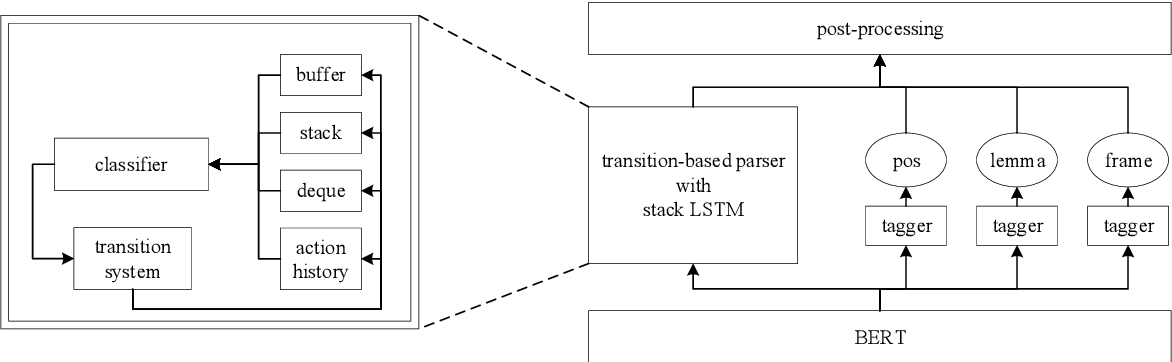
\includegraphics[width=\textwidth]{hitscir1}
\end{center}
\end{frame}


\section{What Distinguishes Meaning Representations?}


\begin{frame}
\frametitle{UCCA vs. UD}

    \begin{minipage}[t]{.17\textwidth}
      \onslide<2->{
        \fbox{Many formal differences.}
      }
    \end{minipage}
    \begin{minipage}{.5\textwidth}
        \scalebox{.77}{
\begin{tikzpicture}[level distance=2cm, sibling distance=25mm, ->, draw=Indigo, thick]
    \node[anchor=west,font=\bf\sffamily\LARGE,Indigo] at (-3,0) {UCCA};
    \node (ROOT) [fill=Indigo, circle] {}
      child {node (After) {After} edge from parent node[left] {L\;}}
      child {node (graduation) [fill=Indigo, circle] {}
      {
        child {node {graduation} edge from parent node[left] {P}}
      } edge from parent node[left] {H} }
      child {node {,} edge from parent node[right] {U}}
      child {node (moved) [fill=Indigo, circle] {}
      {
        child {node (Daniel) {Daniel} edge from parent node[left] {A}}
        child {node {moved} edge from parent node[left] {P}}
        child {node [fill=Indigo, circle] {}
        {
          child {node {to} edge from parent node[left] {R}}
          child {node {Copenhagen} edge from parent node[left] {C}}
        } edge from parent node[left] {A} }
      } edge from parent node[right] {H} }
      ;
    \draw[dashed,->] (graduation) to node [auto] {A} (Daniel);
\end{tikzpicture}
        }
    \end{minipage}
    \begin{minipage}{.2\textwidth}
      \onslide<3->{
        \fbox{What about \textit{content}?}
        \vspace{4cm}
      }
    \end{minipage}
    
    {\color{DarkBlue}\bf\sffamily\Large UD}
    
    \vspace{-14mm}
    
    \rmfamily
    \begin{dependency}[text only label, edge style={-{Latex[length=2mm]}, color=DarkBlue, thick},
                       label style={above, color=DarkBlue, font=\bf\ttfamily}, font=\small]
    \begin{deptext}[column sep=.8em,ampersand replacement=\^]
    After \^ graduation \^ , \^ Daniel \^ moved \^ to \^ Copenhagen \\
    \end{deptext}
        \depedge{2}{1}{case}
        \depedge{2}{3}{punct}
        \depedge{5}{4}{nsubj}
        \depedge[edge end x offset=-2pt]{5}{2}{obl}
        \depedge{7}{6}{case}
        \deproot[edge unit distance=2.5ex]{5}{root}
        \depedge{5}{7}{obl}
    \end{dependency}
\end{frame}


\begin{frame}
\frametitle{Assimilating the Graph Structures}

\begin{minipage}{.04\textwidth}
\color{DarkBlue} UD
\end{minipage}
\only<-2>{
\begin{minipage}{.45\textwidth}
  \centering
  \scalebox{.6}{
    \begin{dependency}[text only label, edge style={color=DarkBlue},
                       label style={above, color=DarkBlue, font=\bf\ttfamily}, font=\small]
    \begin{deptext}[column sep=.8em,ampersand replacement=\^]
    After \^ graduation \^ , \^ Daniel \^ moved \^ to \^ Copenhagen \\
    \end{deptext}
        \depedge{2}{1}{case}
        \depedge{2}{3}{punct}
        \depedge{5}{4}{nsubj}
        \depedge[edge end x offset=-2pt]{5}{2}{obl}
        \depedge{7}{6}{case}
        \deproot[edge unit distance=2.5ex]{5}{root}
        \depedge{5}{7}{obl}
    \end{dependency}
    }
\end{minipage}
\begin{minipage}{.02\textwidth}
\Rightarrow
\end{minipage}
\begin{minipage}{.4\textwidth}
  \centering
  \scalebox{.55}{\convertedudgraduation}
\end{minipage}
}
\only<3->{
\begin{minipage}{.9\textwidth}
  \centering
  \scalebox{.9}{\convertedudgraduation}
\end{minipage}
}

\pause
\vfill

Evaluate by matching edges \citep*{hershcovich2019content}.

\pause
\vfill

\begin{minipage}{.5\textwidth}
\scalebox{.7}{
\begin{tikzpicture}[level distance=17mm, sibling distance=25mm, ->, draw=Indigo, thick]
    \node[anchor=west,font=\sffamily\LARGE,Indigo] at (-4,0) {UCCA};
    \node (ROOT) [fill=Indigo, circle] {}
      child {node (After) {After} edge from parent node[left] {L\;}}
      child {node (graduation) [fill=Indigo, circle] {}
      {
        child {node {graduation} edge from parent node[left] {P}}
      } edge from parent node[left] {H} }
      child {node {,} edge from parent node[right] {U}}
      child {node (moved) [fill=Indigo, circle] {}
      {
        child {node (Daniel) {Daniel} edge from parent node[left] {A}}
        child {node {moved} edge from parent node[left] {P}}
        child {node [fill=Indigo, circle] {}
        {
          child {node {to} edge from parent node[left] {R}}
          child {node {Copenhagen} edge from parent node[left] {C}}
        } edge from parent node[left] {A} }
      } edge from parent node[right] {H} }
      ;
    \draw[dashed,->] (graduation) to node [auto] {A} (Daniel);
\end{tikzpicture}
}
\end{minipage}
\pause
\begin{minipage}[b]{.4\textwidth}
    \large
    \begin{tabular}{c|c|c}
        \textbf{P} & \textbf{R} & \textbf{F1} \\ \hline
        $\frac89=89\%$ & $\frac8{10}=80\%$ & 84\%
    \end{tabular}
    \vspace{1cm}
\end{minipage}
\end{frame}


\begin{frame}
\frametitle{Scenes and non-Scenes, Relations and Participants}
\begin{flushright}
\scalebox{.9}{
\begin{tikzpicture}[level distance=15mm, sibling distance=21mm, ->, draw=Indigo, thick]
    \node[anchor=west,font=\sffamily\LARGE,Indigo] at (-4,0) {UCCA};
    \node (ROOT) [fill=Indigo, circle] {}
      child {node (After) {After} edge from parent node[above] {L\;}}
      child {node (graduation) [fill=Indigo, circle] {}
      {
        child {node {graduation} edge from parent [Indigo] node[left] {P}}
      } edge from parent [alt=<2>{red}{}] node[left] {H} }
      child {node {,} edge from parent node[right] {U}}
      child {node (moved) [fill=Indigo, circle] {}
      {
        child {node (Daniel) {Daniel} edge from parent [alt=<3>{red}{Indigo}] node[above] {A}}
        child {node {moved} edge from parent [Indigo] node[left] {P}}
        child {node [fill=Indigo, circle] {}
        {
          child {node {to} edge from parent [Indigo] node[left] {R}}
          child {node {Copenhagen} edge from parent [Indigo] node[right] {C}}
        } edge from parent [alt=<3>{red}{Indigo}] node[right] {A} }
      } edge from parent [alt=<2>{red}{}] node[above] {H} }
      ;
    \draw[dashed,->] (graduation) to node [auto] {A} (Daniel);
\end{tikzpicture}
}
\end{flushright}

\vspace{-13mm}

{\color{DarkBlue}\Large\sffamily Converted UD}

\vspace{-1mm}

\scalebox{.9}{\convertedudgraduation}
\end{frame}


\begin{frame}
\frametitle{Multi-word Expressions}

\begin{flushright}
\scalebox{.9}{
\begin{tikzpicture}[level distance=15mm, sibling distance=28mm, ->, draw=Indigo, thick,
  level 2/.style={sibling distance=16mm}]
  \tikzstyle{word} = [color=black]
    \node[anchor=west,font=\sffamily\LARGE,Indigo] at (-4,0) {UCCA};
    \node (ROOT) [fill=Indigo, circle] {}
      child {node (They) [word] {They} edge from parent node[above] {A}}
      child {node [word] {thought} edge from parent node[left] {P}}
      child {node (abouttakingashortbreak) [fill=Indigo, circle] {}
      {
        child {node [word] {about} edge from parent [Indigo] node[left] {R}}
        child {node (takingabreak) [fill=Indigo, circle] {}
        {
          child {node [word] {taking} edge from parent [alt=<3>{red}{Indigo}] node[above] {F}}
          child {node [word] {a} edge from parent [alt=<3>{red}{Indigo}] node[right] {F}}
          child {node [word] (short) {short} edge from parent[draw=none]}
          child {node [word] {break} edge from parent [alt=<3>{red}{Indigo}] node[right] {C}}
        } edge from parent [Indigo] node[right] {P} }
      } edge from parent node[above] {A} }
      ;
    \draw[bend left,dashed,->] (abouttakingashortbreak) to node [auto] {A} (They);
    \draw[bend left,->] (abouttakingashortbreak) to node [auto] {D} (short);
\end{tikzpicture}
}
\end{flushright}

\vspace{-12mm}

\only<1>{
    {\color{DarkBlue}\Large\sffamily UD}

     \begin{dependency}[line width=1.5pt]
        \begin{deptext}[column sep=1.5em,ampersand replacement=\^,font=\rmfamily]
       They \^ thought \^ about \^ taking \^ a \^ short \^ break \\
         \end{deptext}
        \deproot[draw=DarkBlue]{2}{root}
        \depedge[draw=DarkBlue]{2}{1}{nsubj}
        \depedge[edge start x offset=-4pt,draw=DarkBlue]{2}{4}{advcl}
        \depedge[draw=DarkBlue]{4}{3}{mark}
        \depedge[draw=DarkBlue]{4}{7}{dobj}
        \depedge[draw=DarkBlue]{7}{5}{det}
        \depedge[draw=DarkBlue]{7}{6}{amod}
    \end{dependency}
}
\only<2->{
  \vspace{-16mm}
    
  {\color{DarkBlue}\Large\sffamily Converted UD}
  
  \scalebox{.9}{
  \begin{tikzpicture}[level distance=17mm, sibling distance=28mm, ->, draw=DarkBlue, thick,
      every node/.append style={sloped,anchor=south,auto=false,font=\scriptsize},
      level 2/.style={sibling distance=19mm},
      edge from parent path={(\tikzparentnode.center) -- (\tikzchildnode.north)}]
    \tikzstyle{word} = [font=\rmfamily,color=black]
    \node (ROOT) [fill=DarkBlue, circle] {}
      child {node (They) [word] {They} edge from parent node {nsubj}}
      child {node [word] {thought} edge from parent node {head}}
      child {node (abouttakingashortbreak) [fill=DarkBlue, circle] {}
      {
        child {node [word] {about} edge from parent node {mark}}
        child {node (takingabreak) [fill=DarkBlue, circle] {}
        {
          child {node [word] {taking} edge from parent node {head}}
          child {node [word] {a} edge from parent node {det}}
          child {node [word] (short) {short} edge from parent node {\;amod}}
          child {node [word] {break} edge from parent node {head}}
        } edge from parent node {dobj} }
      } edge from parent node {advcl} }
      ;
  \end{tikzpicture}
  }
}
\end{frame}


\begin{frame}
\frametitle{Linkage between Scenes}

\begin{flushright}    
    \scalebox{.8}{
    \begin{tikzpicture}[level distance=15mm, sibling distance=39mm, ->, draw=Indigo, thick,
  level 2/.style={sibling distance=16mm},
  every circle node/.append style={fill=Indigo}]
  \tikzstyle{word} = [color=black]
    \node[anchor=west,font=\sffamily\LARGE,Indigo] at (-6,0) {UCCA};
      \node (ROOT) [circle] {}
        child {node [circle] {}
        {
          child {node [word] {From} edge from parent [Indigo] node[left] {R}}
          child {node [word] {the} edge from parent [Indigo] node[left] {E}}
          child {node [word] {{\color{white}F}\color{black}moment} edge from parent [Indigo] node[right] {C}}
        } edge from parent [alt=<2>{red}{}] node[above] {L} }
        child {node [circle] {}
        {
          child {node [word] {you{\color{white}k}} edge from parent node[left] {A}}
          child {node [word] {{\color{white}y}enter} edge from parent node[right] {P}}
        } edge from parent node[left] {H} }
        child {node [circle] {}
        {
          child {node (comma) [word] {,} edge from parent [draw=none]}
          child {node [word] {you{\color{white}k}} edge from parent node[left] {A}}
          child {node [word] {{\color{white}y}know} edge from parent node[right] {S}}
        } edge from parent node[above] {H} }
        ;
      \draw[->] (ROOT) to node [right] {U} (comma);
    \end{tikzpicture}
    }
\end{flushright}

    {\color{DarkBlue}\Large\sffamily UD}
    
    \vspace{-5mm}
    
    \begin{dependency}[line width=1.5pt]
        \begin{deptext}[column sep=1.5em,ampersand replacement=\^,font=\rmfamily]
        From \^ the \^ moment \^ you \^ enter \^ , \^ you \^ know \\
        \end{deptext}
        \depedge[draw=DarkBlue]{3}{1}{case}
        \depedge[draw=DarkBlue]{3}{2}{det}
        \depedge[draw=DarkBlue]{8}{3}{obl}
        \depedge[draw=DarkBlue]{3}{5}{acl}
        \depedge[draw=DarkBlue,edge start x offset=-5pt]{5}{4}{nsubj}
        \depedge[draw=DarkBlue]{8}{6}{punct}
        \depedge[draw=DarkBlue,edge start x offset=-10pt]{8}{7}{nsubj}
        \deproot[draw=DarkBlue]{8}{root}
    \end{dependency}
\end{frame}


\begin{frame}
\frametitle{Confusion Matrix: EWT Reviews Gold Data}
\centering
\setlength\tabcolsep{1pt}
\def\arraystretch{.5}
\scalebox{.7}{
\begin{tabular}{lRRRRRRRRRRRRRRRR|R}
 &&&&&&&&&&&&&&&&& \multicolumn{1}{|c}{\textsc{No}} \\
 & \multicolumn{1}{c}{\textbf{A}}
 & \multicolumn{1}{c}{\textbf{A\big|P}} & \multicolumn{1}{c}{\textbf{A\big|S}}
 & \multicolumn{1}{c}{\textbf{C}}
 & \multicolumn{1}{c}{\textbf{D}}
 & \multicolumn{1}{c}{\textbf{E}}
 & \multicolumn{1}{c}{\textbf{F}}
 & \multicolumn{1}{c}{\textbf{G}}
 & \multicolumn{1}{c}{\textbf{H}}
 & \multicolumn{1}{c}{\textbf{L}}
 & \multicolumn{1}{c}{\textbf{N}}
 & \multicolumn{1}{c}{\textbf{P}}
 & \multicolumn{1}{c}{\textbf{Q}}
 & \multicolumn{1}{c}{\textbf{R}}
 & \multicolumn{1}{c}{\textbf{S}}
 & \multicolumn{1}{c}{\textbf{T}}
 & \multicolumn{1}{|c}{\textsc{Match}} \\
\texttt{acl} & 58 &  &  & 1 & 4 & 249 & 1 &  & 48 &  &  & 6 &  &  & 1 & 1 & 409 \\
\texttt{advcl} & 14 &  &  & 12 & 2 & 2 &  & 6 & 512 & 4 &  & 11 &  &  &  &  & 423 \\
\texttt{advmod} & 225 &  & 1 & 69 & 1778 & 332 & 27 & 135 & 14 & 258 & 2 & 2 & 15 & 44 & 9 & 368 & 273 \\
\texttt{amod} & 25 &  &  & 134 & 647 & 837 &  & 1 & 28 &  &  & 7 & 130 & 3 & 269 & 25 & 176 \\
\texttt{appos} & 21 &  &  & 39 & 2 & 34 &  &  & 18 &  &  &  &  &  & 8 &  & 33 \\
\texttt{aux} &  &  &  &  & 384 & 2 & 1335 &  &  & 2 &  & 1 &  & 1 &  &  & 17 \\
\texttt{case} & 11 &  &  & 31 & 27 & 25 & 123 &  &  & 213 & 26 & 11 & 1 & 2629 & 154 & 1 & 262 \\
\texttt{cc} &  &  &  & 8 & 4 & 1 & 4 & 1 & 1 & 1567 & 381 &  & 6 & 12 &  &  & 52 \\
\texttt{ccomp} & 345 &  &  & 1 &  & 1 &  &  & 36 &  &  & 2 &  &  & 1 & 1 & 166 \\
\texttt{compound} & 225 &  &  & 116 & 67 & 586 & 21 &  & 2 &  &  & 32 & 19 & 1 & 12 & 24 & 683 \\
\texttt{conj} & 10 &  &  & 449 & 4 & 5 &  & 1 & 1262 & 1 &  & 6 & 2 &  & 10 &  & 497 \\
\texttt{cop} &  &  &  & 1 &  &  & 1312 &  &  & 1 &  & 9 &  & 10 & 178 &  & 7 \\
\texttt{csubj} & 13 &  &  &  &  &  &  &  & 3 &  &  &  &  &  &  &  & 46 \\
\texttt{det} & 10 &  &  & 17 & 119 & 440 & 2963 &  &  &  & 1 &  & 129 & 16 & 1 &  & 124 \\
\texttt{discourse} & 1 &  &  & 2 & 1 &  & 25 & 29 & 27 & 16 &  &  &  &  & 5 &  & 19 \\
\texttt{expl} & 21 &  &  & 1 &  &  & 98 &  &  &  &  &  &  &  & 17 &  & 3 \\
\texttt{iobj} & 131 &  &  & 1 &  &  & 1 &  &  &  &  &  &  &  &  &  & 10 \\
\texttt{list} & 3 &  &  & 7 & 2 & 1 &  &  & 27 &  &  &  &  &  & 1 &  & 6 \\
\texttt{mark} &  &  &  & 9 & 7 & 1 & 531 & 1 &  & 654 &  &  &  & 407 & 1 & 5 & 143 \\
\texttt{nmod} & 844 & 1 & 1 & 20 & 9 & 786 & 8 & 4 & 12 & 1 & 1 & 20 & 2 & 2 & 11 & 27 & 488 \\
\texttt{nsubj} & 4296 & 7 & 21 & 25 & 3 & 2 & 55 & 1 & 5 & 61 &  & 58 & 1 & 80 & 14 & 4 & 247 \\
\texttt{nummod} & 2 &  &  & 33 & 12 & 17 &  & 4 &  & 4 &  &  & 334 &  &  &  & 64 \\
\texttt{obj} & 1845 &  & 1 & 54 & 21 & 6 & 11 & 1 & 4 & 23 &  & 52 & 1 & 23 & 3 & 11 & 583 \\
\texttt{obl} & 1195 &  &  & 19 & 115 & 41 & 1 & 17 & 39 & 34 &  & 6 & 6 & 26 & 7 & 302 & 611 \\
\texttt{parataxis} & 6 &  & 1 & 5 &  & 4 &  & 6 & 285 &  &  &  &  &  & 3 &  & 180 \\
\texttt{vocative} & 17 &  &  &  &  &  &  & 8 &  &  &  &  &  &  &  &  &  \\
\texttt{xcomp} & 121 &  &  & 4 & 25 &  &  &  & 8 &  &  & 38 &  &  & 38 &  & 526 \\
\hline
head & 445 & 48 & 159 & 6388 & 717 & 142 & 564 & 83 & 2462 & 42 & 1 & 4163 & 120 & 52 & 1547 & 32 & 2235 \\
\hline
\textsc{No Match} & 1421 & 37 & 58 & 640 & 417 & 291 & 14 & 33 & 2291 & 146 & 6 & 802 & 94 & 52 & 369 & 96 & 
\end{tabular}
}
\end{frame}

\pgfplotstableread{
colnames 1 2 3 4 5 6 7 8 9 10 11 12 13 14 15 16 17 18 19 20 21 22 23 24 25 26 27 28
deprel aux det cop cc expl iobj nsubj case list advmod amod nummod mark vocative compound obj nmod conj advcl obl xcomp discourse ccomp parataxis appos acl csubj {}
lf 94 93 89 86 83 83 80 76 76 72 71 71 70 62 59 57 55 50 49 48 41 38 29 23 21 20 0 0
uf 99 99 100 99 100 83 84 95 76 95 95 86 97 92 84 65 77 61 51 61 63 95 29 36 48 37 33 0
}\finegrained
\pgfplotstabletranspose[colnames from=colnames]\finegrainedtranspose{\finegrained}

\begin{frame}
\frametitle{Fine-grained UCCA Parsing Evaluation}
        \begin{tikzpicture}
        \begin{axis}[
        ybar,
        bar width=1,
        enlarge x limits=0,
        ymin=0,
        clip=true,
        width=\textwidth,
        height=.8\textheight,
        xtick=data,
        xticklabels from table={\finegrainedtranspose}{deprel},
        ylabel={TUPA F1 (\%)},
        y label style={at={(1.15,.5)}},
        legend style={at={(1.075,.975)}},
        xticklabel style={rotate=90},
        tick label style={font=\scriptsize},
        xticklabel style={anchor=north east},
        ]
        \addplot+[area legend,ybar interval] table [y=uf,x expr=\coordindex] {\finegrainedtranspose};
        \addplot+[area legend,ybar interval] table [y=lf,x expr=\coordindex] {\finegrainedtranspose};
        \legend{Unlabeled,Labeled};
        \end{axis}
        \end{tikzpicture}
\end{frame}


\begin{frame}
\frametitle{Ongoing Work}

Complement syntax with \textit{lexical} semantics to make up for differences.

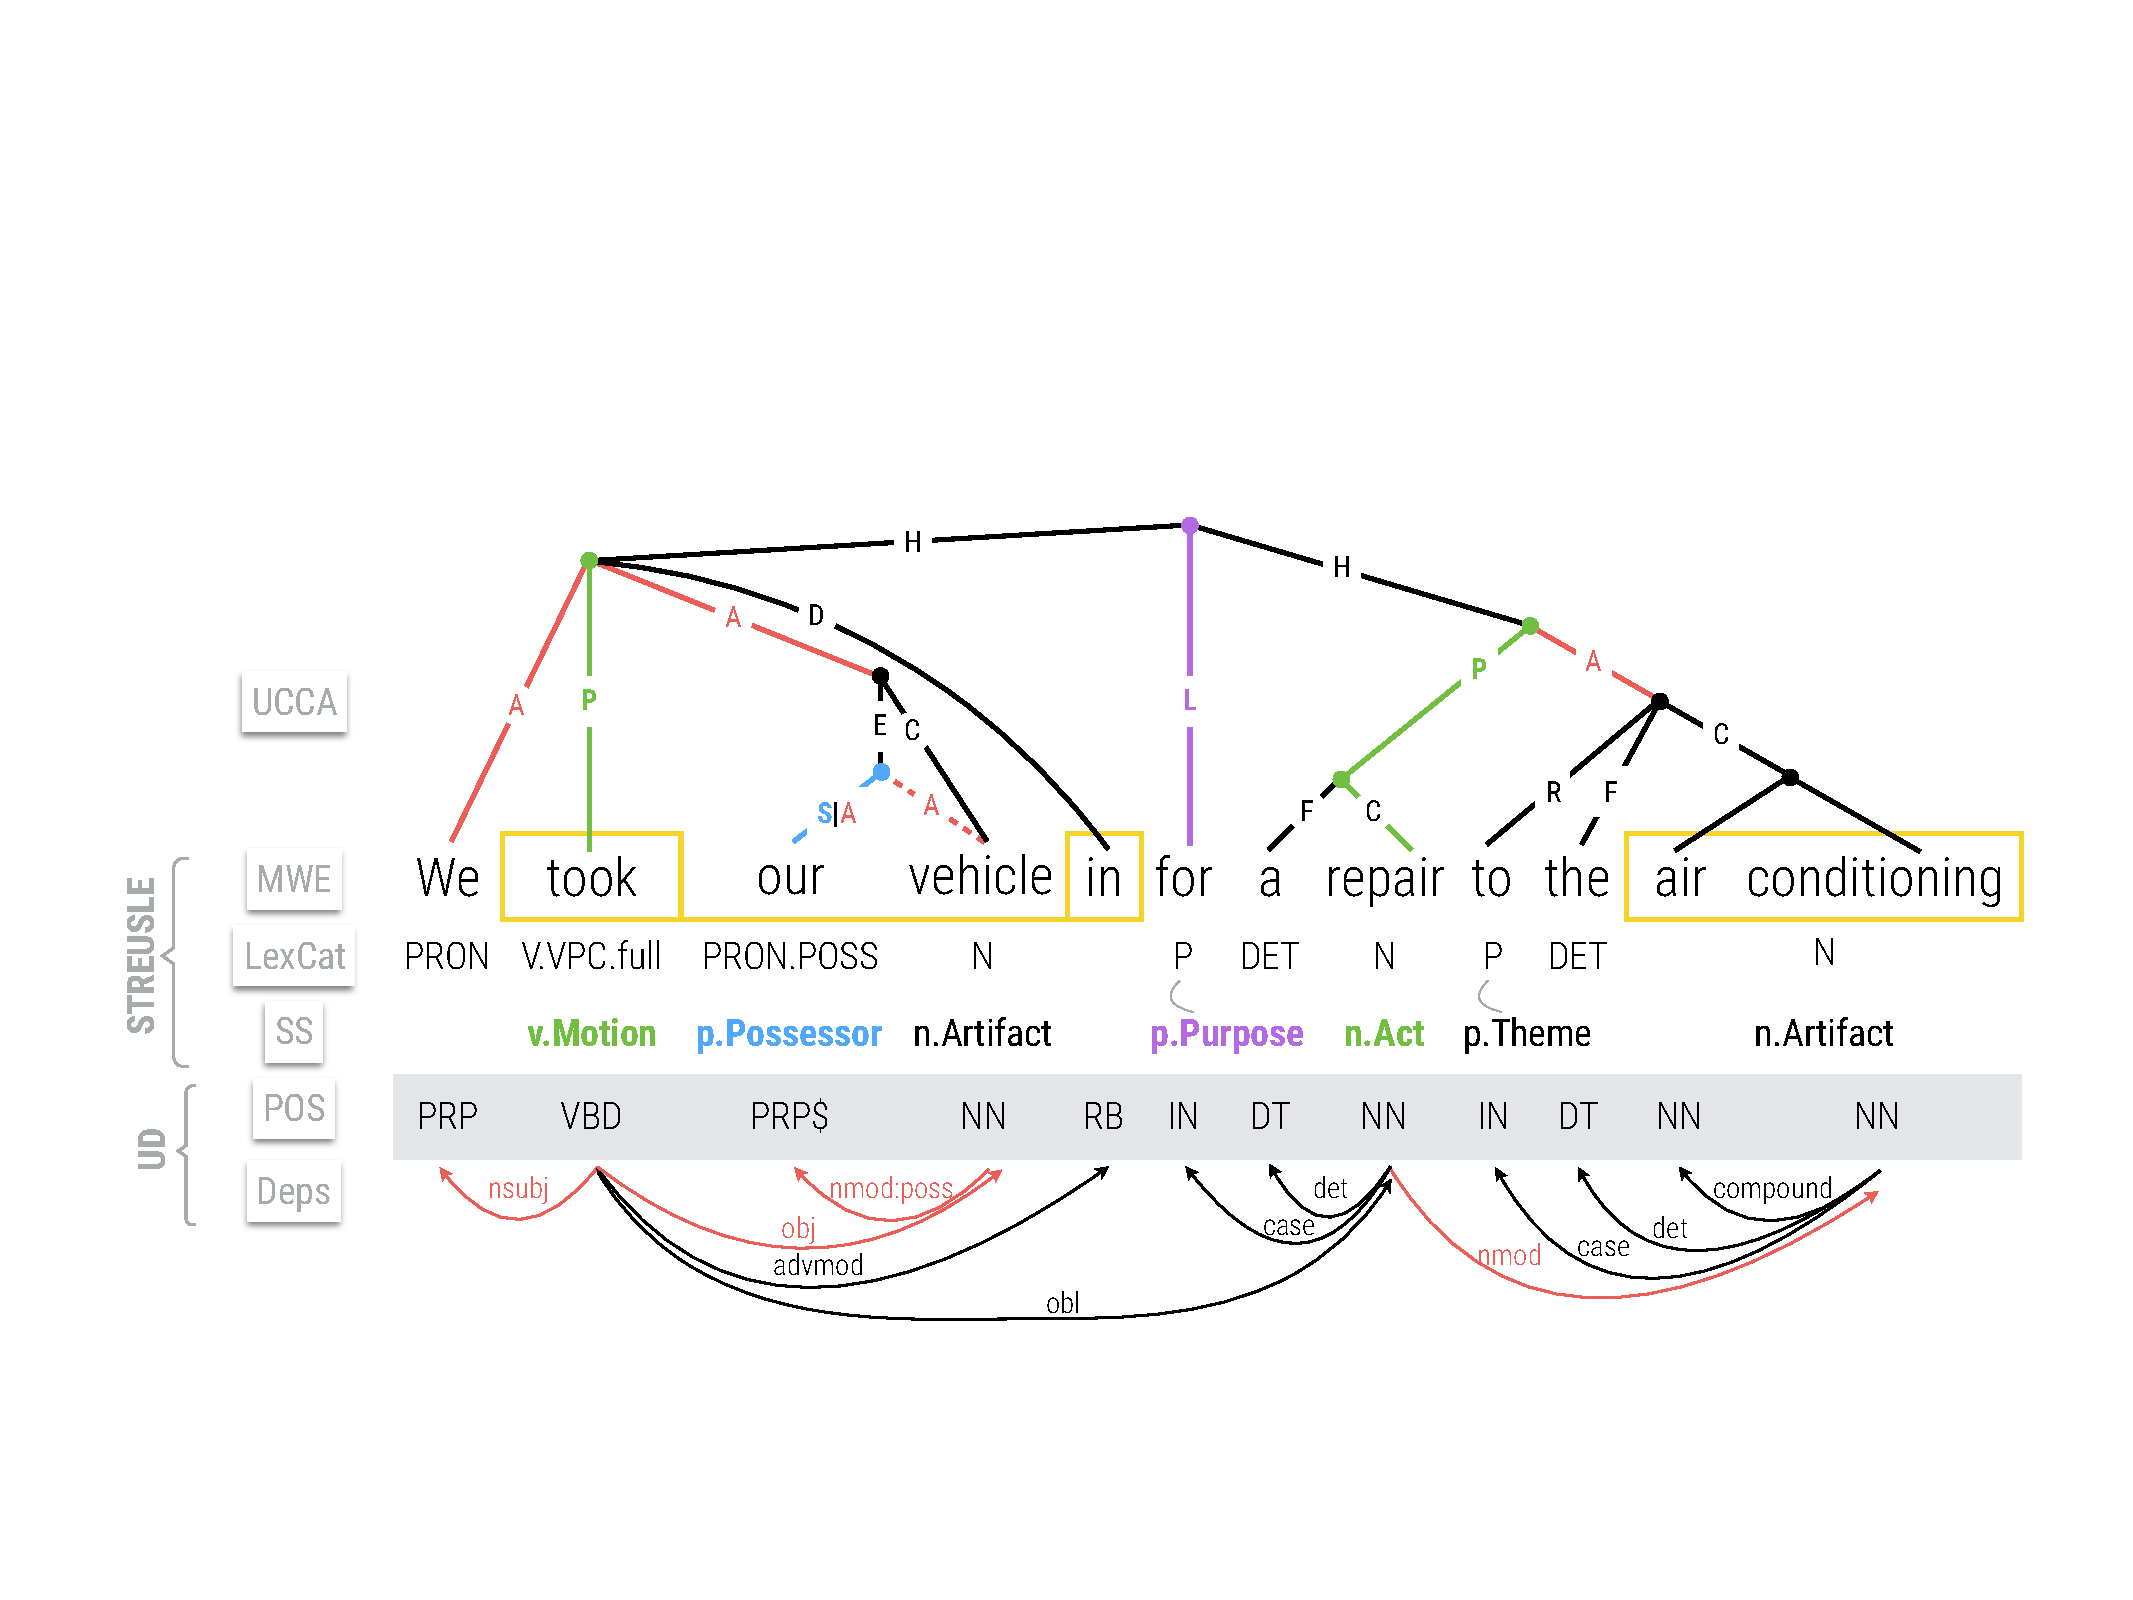
\includegraphics[width=\textwidth]{ex-ucca-streusle.pdf}

\end{frame}



\section*{}

\begin{frame}
\frametitle{Conclusion}
\begin{itemize}
 \item Meaning representation is valuable for language understanding.\pause
 \item Transition-based parsers excel across frameworks and languages.\pause
 \item Cross-framework unification by multi-task and linguistic analysis.\pause
\end{itemize}

\vfill
\begin{minipage}{.8\textwidth}
\begin{adjustbox}{scale=.6}
            \begin{tikzpicture}[level distance=7mm, sibling distance=6mm,
                every node/.append style={font=\rmfamily},
            	every circle node/.append style={fill=Indigo}]
                \begin{scope}[frontier/.style={distance from root=23mm},
                    edge from parent path={(\tikzparentnode.center)
                	.. controls +(0,-.25) and +(0,.25) .. (\tikzchildnode.north)},
                    edge from parent/.append style={nodes={font=\scriptsize}}]
                \Tree [.\node [circle] (root u) {};
                  \edge node [auto=right]{L}; \node (After u) {After};
                  \edge node[auto=left]{H};
                  [.\node [circle,xshift=8mm](graduation Daniel u) {};
                    \edge node[auto=right]{P}; \node (graduation u) {graduation};
                  ]
                  \edge node[auto=left]{H};
                  [.\node [circle](Daniel moved to Copenhagen u) {};
                    \edge node[auto=right]{A}; \node (Daniel u) {Daniel};
                    \edge node[auto=left]{P}; \node (moved u) {moved};
                    \edge node[auto=left]{A};
                    [.\node [circle](to Copenhagen u) {};
                      \edge node[auto=right]{R}; \node (to u) {to};
                      \edge node[auto=left]{C}; \node (Copenhagen u) {Copenhagen};
                    ]
                  ]
                ]
                \draw[dashed] (graduation Daniel u) to node[auto,style={font=\scriptsize}] {A} (Daniel u);
                \end{scope}
                \onslide<2->{
                  \begin{scope}[xshift=2cm,yshift=-58mm,grow'=up,level distance=9mm,
                      sibling distance=4mm, frontier/.style={distance from root=19mm},
                      edge from parent path={(\tikzparentnode.center) ..
                      controls +(0,.25) and +(0,-.25) .. (\tikzchildnode.south)},
                      edge from parent/.append style={nodes={font=\scriptsize}}]
                  \Tree [.\node [circle] (rootd) {};
                    \edge node[auto=left]{H};
                    [.\node [circle,xshift=-5mm] (Daniel siyem et halimudim d) {};
                      \edge node[auto=left]{P}; \node (halimudim d) {\heb{הלימודים}};
                      \edge node[auto=left]{F}; \node (et d) {\heb{את}};
                      \edge node[auto=right]{D}; \node (siyem d) {\heb{שסיים}};
                    ]
                    \edge node [auto=left,anchor=south east]{L}; \node (ahrei d) {\heb{אחרי}};
                    \edge node[auto=right]{H};
                    [.\node [circle] (hu avar lecopenhagen d) {};
                      \edge node[auto=left,anchor=south east]{A}; \node (lecopenhagen d) {\heb{לקופנהגן}};
                      \edge node[auto=left]{P}; \node (avar d) {\heb{עבר}};
                      \edge node[auto=right]{A}; \node (Daniel d) {\heb{דניאל}};
                    ]
                  ]
                  \draw[dashed] (Daniel siyem et halimudim d) to[out=-15,in=-150] node[above,style={font=\scriptsize}] {A} (Daniel d);
                  \end{scope}
                }
                  \begin{scope}[dashed,thick]
                    \draw[DarkRed] (After u) to[out=-45,in=135] (ahrei d);
                    \draw[DarkGreen] (graduation u) to[out=-90,in=100] (Daniel siyem et halimudim d);
                    \draw[DarkBlue] (Daniel u) -- (Daniel d);
                    \draw[orange] (moved u) to[out=-30,in=90] (avar d);
                    \draw[magenta] (to Copenhagen u) to[out=-90,in=70] (lecopenhagen d);
                  \end{scope}
            \end{tikzpicture}
\end{adjustbox}
\end{minipage}
\begin{minipage}{.15\textwidth}
Thanks!
\end{minipage}

\end{frame}

\begin{frame}[allowframebreaks]
\frametitle{References}
\bibliographystyle{plainnat}
\tiny\bibliography{references}
\end{frame}

\end{document}
